\documentclass[12pt,a4paper]{report}

% ─── Pakete ────────────────────────────────────────────────────────────────────
\usepackage[utf8]{inputenc}
\usepackage[T1]{fontenc}
\usepackage[ngerman]{babel}
\usepackage{geometry}

\usepackage{amsmath, amssymb, amsthm, mathtools}
\usepackage{graphicx}
\usepackage{booktabs}
\usepackage{array}
\usepackage{longtable}
\usepackage{hyperref}
\usepackage{xcolor}
\usepackage{enumitem}
\usepackage{setspace}
\usepackage{textcomp}
\usepackage{caption}
\captionsetup{singlelinecheck=false}
\usepackage{fancyhdr}
\usepackage{parskip}
\usepackage[expansion=false,protrusion=true]{microtype}
\setlength{\emergencystretch}{1em}
\usepackage{tikz}
\usetikzlibrary{arrows.meta, positioning, shapes.geometric, fit, backgrounds}

\setlist[itemize,1]{label=--}

% ─── Layout ────────────────────────────────────────────────────────────────────
\geometry{margin=2.5cm, headheight=15pt}

\hypersetup{colorlinks=true, linkcolor=[rgb]{0.0,0.3,0.6},
	citecolor=[rgb]{0.0,0.3,0.6}, urlcolor=[rgb]{0.0,0.3,0.6}}

% ─── Theorem-Umgebungen ────────────────────────────────────────────────────────
\theoremstyle{plain}
\newtheorem{theorem}{Theorem}[section]
\newtheorem{lemma}[theorem]{Lemma}
\newtheorem{korollar}[theorem]{Korollar}
\newtheorem{proposition}[theorem]{Proposition}

\theoremstyle{definition}
\newtheorem{definition}[theorem]{Definition}
\newtheorem{experiment}[theorem]{Experiment}
\newtheorem{axiom}[theorem]{Axiom}
\newtheorem{beobachtung}[theorem]{Beobachtung}

\theoremstyle{remark}
\newtheorem{bemerkung}[theorem]{Bemerkung}
\newtheorem{beispiel}[theorem]{Beispiel}

% ─── Mathe-Operatoren ──────────────────────────────────────────────────────────
\DeclareMathOperator{\MHI}{MHI}
\DeclareMathOperator{\GHI}{GHI}
\DeclareMathOperator{\GC}{GC}
\DeclareMathOperator{\ITR}{ITR}
\DeclareMathOperator{\PAC}{PAC}
\DeclareMathOperator{\sgn}{sgn}
\DeclareMathOperator{\MI}{MI}
\DeclareMathOperator{\EMG}{EMG}

\title{\textbf{Die Hand als primäres Werkzeug des Geistes}\\[0.5em]
\large Neuroanatomische, biomechanische, informationstheoretische und\\
evolutionäre Formalisierung der manuellen Suprematie}
\author{Stephan Epp}
\date{5. April 2026}

% ══════════════════════════════════════════════════════════════════════════════
\begin{document}
\pagenumbering{roman}
\maketitle
\tableofcontents
\newpage
\pagenumbering{arabic}

% ══════════════════════════════════════════════════════════════════════════════
\chapter{Einleitung}
% ══════════════════════════════════════════════════════════════════════════════

Die menschliche Hand ist weit mehr als ein mechanisches Greiforgan.
Sie ist -- neurologisch, informationstheoretisch und evolutionär betrachtet --
das komplexeste und bedeutsamste periphere Organ des menschlichen Körpers,
das in permanenter bidirektionaler und hochbandbreitiger Kommunikation
mit den höchsten Instanzen des Zentralnervensystems steht. Die zentrale Aussage
dieser Arbeit lautet:

\begin{quote}
\textit{Die Hand des Menschen ist das wichtigste Werkzeug nicht nur
körperlicher, sondern geistiger Arbeit. Ihre sensorische Bandbreite,
ihre kortikale Dominanz, ihre evolutionäre Formgebung und ihre Rolle
als bidirektionale Schnittstelle zwischen Geist und Welt machen sie zum
primären Organ menschlicher Handlungsfähigkeit -- und damit zur
notwendigen Bedingung für Gesundheit, Kognition und Wohlbefinden des
Menschen.}
\end{quote}

Diese Aussage ist keine metaphorische Ãœberspitzung. Sie ist eine biologisch
präzise Aussage, die sich aus der Neuroanatomie, der Regelungstheorie,
der Informationstheorie, der Evolutionsbiologie und der klinischen Medizin
gleichermaßen ableiten lässt. Das Gehirn -- die epistemische Wolke unserer
Gedanken \cite{epp2026brn} -- ist ohne manuelle Ausgabe ein blindes
Rechenzentrum ohne Wirkung in der Welt. Die Hand ist der primäre Effektor
des Willens. Die Hand ist zugleich der sekundäre Sensor der Welt.
Sie schreibt, greift, tastet, erschafft, kommuniziert, heilt.

Die vorliegende Abhandlung steht in direkter thematischer Verwandtschaft
zu den Arbeiten des Autors über den Fuß als sensorisches Primärorgan
\cite{epp2026feed}, über den Gluteus-Grundsatz der posturalen Integrität
\cite{epp2026butt} sowie über kortikale Rechtsdrehung und den unsichtbaren
Geist des Lebens \cite{epp2026brn}. Der Fuß liefert die propriozeptive
Grundlage des Körperschemas; das Gesäß stabilisiert die posturale Plattform;
das Gehirn verarbeitet -- rechtsdrehend, selektiv, in epistemischer Freiheit
oder Wolke. Die Hand jedoch ist das Organ, das all diese Systeme in
\emph{Wirkung} übersetzt. Sie schließt den Regelkreis zwischen Geist und Welt.

Die vorliegende Abhandlung vereint acht fundamentale Argumente zu einem
kohärenten theoretischen Rahmen, belegt durch \textbf{neun Klassen
computergestützter Modellexperimente mit insgesamt 34 Teildiagrammen},
begleitet von \textbf{neun Theoremen mit vollständigen Beweisen},
\textbf{sieben Definitionen}, \textbf{vier Axiomen} und
\textbf{drei formalen Propositionen}.

\textbf{Schlüsselwörter:}
Hand, Mechanorezeption, somatosensorischer Kortex, motorischer Homunkulus,
Greifbiomechanik, Feinmotorik, Fitts-Gesetz, Handgreifkraft, Mortalitätsprädiktor,
kortikale Neuroplastizität, Musiker-Gehirn, Parkinson-Tremor,
Karpaltunnelsyndrom, Informationstheorie, Granger-Kausalität,
Phase-Amplitude-Kopplung, manueller Gesundheitsindex, Handschrift, Kognition

\section{Hintergrund und Problemstellung}

Der menschliche Körper ist -- wie in den parallelen Arbeiten des Autors
eingehend dargelegt -- ein hierarchisches Regelwerk, dessen Qualität
von der Güte seiner Sensoren und Effektoren abhängt. Während der Fuß
\cite{epp2026feed} die propriozeptive Basis der Standregulation liefert
und das Gesäß \cite{epp2026butt} die posturale Plattform stabilisiert,
ist die Hand das Organ, das den Organismus mit der kulturellen und
physischen Welt verbindet.

Die Hand des Homo sapiens ist das Produkt von sechs Millionen Jahren
Evolution, in deren Verlauf die Befreiung der oberen Extremität vom
Gehstütz durch den aufrechten Bipedismus eine explosionsartige
Spezialisierung ermöglichte: präziser Pinch-Griff, kraftvoller
Faustschluss, opponierender Daumen, höchste Mechanorezeptordichte im
gesamten Körper. Diese Spezialisierung ist kein Zufall. Sie ist das
neuronale und mechanische Korrelat kognitiver Komplexität.

\begin{beobachtung}
Die kortikale Repräsentation der Hand im somatosensorischen Kortex (S1)
und im primären Motorkortex (M1) umfasst zusammen mehr als 35\,\% der
gesamten Kortexfläche beider Karten -- obwohl die Hand weniger als 1\,\%
der Körperoberfläche ausmacht.
\end{beobachtung}

Diese Beobachtung -- die kortikale Überrepräsentation der Hand -- ist der
Ausgangspunkt der vorliegenden Arbeit. Sie quantifiziert, formalisiert und
beweist, warum die Hand das wichtigste Organ menschlichen Arbeitens und
Denkens ist.

% ══════════════════════════════════════════════════════════════════════════════
\chapter{Neuroanatomische Grundlagen: Die Hand als sensorisches Organ}
\label{chap:neuroanatomie}
% ══════════════════════════════════════════════════════════════════════════════

\section{Anatomie der Handinnenfläche und Fingerkuppen}

Die Handinnenfläche und insbesondere die Fingerkuppen des Menschen sind
ein anatomisches Wunder der sensorischen Dichte. Auf einer Gesamtfläche
von durchschnittlich 180--220\,cm² beherbergt die Hand vier Klassen von
Mechanorezeptoren, deren Kombination ein sensorisches Ensemble von
einzigartiger Leistungsfähigkeit bildet.

\begin{definition}[Mechanorezeptorklassen der Hand]
Die Handinnenfläche enthält vier primäre kutane Mechanorezeptortypen:
\begin{enumerate}
\item \textbf{Meissner-Körperchen (RA1):} Schnell adaptierende Rezeptoren
  in den dermalen Papillen der Finger. Sensibel für leichten Berührungsdruck
  und Vibration (10--50\,Hz). Dichte an der Fingerkuppe: ca.\,140\,Rezeptoren/cm².
\item \textbf{Pacini-Körperchen (RA2):} Sehr schnell adaptierende Rezeptoren.
  Sensibel für Hochfrequenzvibration (200--300\,Hz); vermitteln das Gefühl
  von Oberflächenrauheit beim Gleiten. Dichte: ca.\,25/cm².
\item \textbf{Merkel-Scheiben (SA1):} Langsam adaptierende Rezeptoren.
  Sensibel für statischen Druck und Kantendetektion; essenziell für
  das Lesen von Braille-Schrift. Dichte: ca.\,180/cm².
\item \textbf{Ruffini-Körperchen (SA2):} Sehr langsam adaptierende Rezeptoren.
  Sensibel für Dehnung und Fingerstellung; konstituieren die prädominante
  Propriozeptionsquelle des Fingers. Dichte: ca.\,30/cm².
\end{enumerate}
\end{definition}

Hinzu kommen propriozeptive Rezeptoren in der Handmuskulatur
(Ia- und Ib-Afferenzen aus Muskelspindeln und Golgi-Sehnenorganen der
intrinsischen Handmuskeln), Gelenkafferenzen (Ruffini-ähnliche Körperchen
in Kapsel und Bändern) sowie freie Nervenendigungen (A$\delta$- und C-Fasern).

\begin{beobachtung}
Die Zwei-Punkt-Diskriminierungsschwelle der Fingerkuppe beträgt
2--3\,mm -- vergleichbar nur mit der Zungenspitze (1--2\,mm) und
signifikant kleiner als Fußsohle (11--14\,mm), Unterarm (30--40\,mm)
oder Rücken (50--60\,mm). Diese Schwelle korreliert direkt mit der
räumlichen Auflösung der kortikalen Karte und belegt die
außergewöhnliche sensorische Präzision der Fingerkuppe.
\end{beobachtung}

\section{Die aufsteigende sensorische Bahn der Hand}

Die afferenten Impulse aus der Hand durchlaufen folgende Stationen,
die in ihrer topographischen Ordnung die Präzision der Fingersensorik
erhalten:

\begin{enumerate}
\item \textbf{Periphere Nervenfasern (N.\ medianus, N.\ ulnaris, N.\ radialis):}
  Leitungsgeschwindigkeit 40--80\,m/s (A$\beta$) bis 1--2\,m/s (C-Fasern).
  Die schnellen A$\beta$-Fasern der Touchrezeptoren leiten mit bis zu 80\,m/s.
\item \textbf{Hinterhorn des Rückenmarks (C6--T1):} Erste synaptische
  Umschaltung. Der kurze Weg Hand--Rückenmark ($\sim$0{,}8\,m) ermöglicht
  spinale Reflexlatenzen von ca.\,10\,ms.
\item \textbf{Nucleus cuneatus (Medulla oblongata):} Zweite Umschaltung.
  Kreuzung zur Gegenseite im Lemniscus medialis. Somatotope Ordnung bleibt
  erhalten: Radiale Finger lateral, ulnare Finger medial.
\item \textbf{Thalamus (VPLc, VPM):} Dritte Umschaltung. Die Hand-Repräsentation
  im VPLc ist flächenmäßig die größte im Thalamus.
\item \textbf{Primärer Sensorikortex (S1, Area 3b/1/2):} Kortikale Repräsentation.
  Die Hand liegt lateral am Sulcus centralis -- leicht zugänglich für
  ECoG und direkte kortikale Stimulation.
\item \textbf{Sekundärer Sensorikortex (S2), Insel, parietaler posteriorer Kortex:}
  Höhere Integration; taktile Objekterkennung, Griff-Kraftkontrolle.
\end{enumerate}

\begin{axiom}[Vollständigkeit des sensorischen Aufwärtspfades der Hand]
\label{ax:vollstaendigkeit}
Jede sensorische Information der Hand, die das Rückenmark erreicht, wird
bei intaktem Nervensystem dem Kortex präsentiert. Es gibt keinen
sensorischen Eingang aus der Hand, der das Gehirn vollständig umgeht.
\end{axiom}

% ══════════════════════════════════════════════════════════════════════════════
\chapter{Der somatosensorische und motorische Homunkulus}
\label{chap:homunkulus}
% ══════════════════════════════════════════════════════════════════════════════

\section{Penfieldsche Kartierung und kortikale Repräsentation}

Wilder Penfield und Theodore Rasmussen kartierten 1950 durch direkte
kortikale Elektrostimulation die somatotope Repräsentation im primären
Sensorik- (S1) und Motorkortex (M1). Das resultierende Bild -- der
\emph{Homunkulus} -- offenbart eine dramatische Überrepräsentation der Hand:
Finger und Hand allein beanspruchen mehr kortikale Fläche als Rumpf,
Beine und innere Organe zusammen.

\begin{theorem}[Kortikale Überrepräsentation der Hand]
\label{thm:homunkulus}
Sei $A_{\mathrm{S1}}(r)$ die kortikale Fläche, die der Körperregion $r$
im primären Sensorikortex (Area 3b) zugewiesen ist. Dann gilt:
\[
  A_{\mathrm{S1}}(\text{Finger}) + A_{\mathrm{S1}}(\text{Hand})
  > A_{\mathrm{S1}}(\text{Rumpf}) + A_{\mathrm{S1}}(\text{Bein}) +
    A_{\mathrm{S1}}(\text{Schulter}) + A_{\mathrm{S1}}(\text{Hüfte})
\]
\end{theorem}

\begin{proof}
Aus den neuroanatomischen Daten von Penfield \& Rasmussen \cite{penfield1950}
ergibt sich:
\begin{align*}
  A_{\mathrm{S1}}(\text{Finger}\,{+}\,\text{Hand}) &\approx 13{,}6\;\text{rel.E.}\\
  A_{\mathrm{S1}}(\text{Rumpf}\,{+}\,\text{Bein}\,{+}\,\text{Schulter}\,{+}\,\text{Hüfte})
    &\approx 7{,}4\;\text{rel.E.}
\end{align*}
Da $13{,}6 > 7{,}4$, ist die Behauptung bewiesen. Finger und Hand allein
belegen fast $1{,}84\times$ die kortikale Fläche des gesamten Rumpf-Bein-Komplexes.
\end{proof}

\begin{figure}[ht]
\centering

\includegraphics[width=\textwidth]{fig01_homunkulus.pdf}
\caption{Links: Kortikale Repräsentationsflächen im somatosensorischen
Homunkulus (blau, S1) und motorischen Homunkulus (grün, M1) für verschiedene
Körperregionen. Die rot hervorgehobenen Finger- und Handareale dominieren
mit zusammen ca.\ 13{,}6 relativen Einheiten. Rechts: Der kortikale
Magnifikationsfaktor $\varrho_{\mathrm{S1}}(r) = A_{\mathrm{S1}}(r) / A_{\mathrm{K\ddot{o}rper}}(r)$
pro Flächeneinheit. Die Fingerkuppen weisen mit Abstand den höchsten Wert
auf: über 240-mal höher als der Rücken. Dies ist keine evolutionäre
Verschwendung, sondern der neuronale Ausdruck der sensorischen und motorischen
Bedeutung der Hand für den Menschen.}
\label{fig:homunkulus}
\end{figure}

Das linke Panel von Abbildung~\ref{fig:homunkulus} vergleicht S1- und
M1-Flächen. Bemerkenswert ist die Kohärenz beider Karten: Die Hand ist
sowohl sensorisch als auch motorisch überproportional repräsentiert,
was die doppelte Funktion als Sensor und Effektor widerspiegelt.
Das rechte Panel zeigt den Magnifikationsfaktor -- also die kortikale
Fläche pro cm² Körperoberfläche. Die Fingerkuppe erreicht hier
astronomische Werte von mehr als 2,0 -- relativ zu anderen Regionen.
Kein anderes Körperteil kommt auch nur annähernd an diese Werte heran.

\section{Quantitative Analyse: Kortikaler Magnifikationsfaktor}

\begin{definition}[Kortikaler Magnifikationsfaktor]
\label{def:magnifikation}
Sei $\varrho_{\mathrm{S1}}(r) = A_{\mathrm{S1}}(r) / A_{\mathrm{K\ddot{o}rper}}(r)$
der \emph{kortikale Magnifikationsfaktor} der Körperregion $r$, gemessen
in relativen Einheiten pro cm² Körperoberfläche.
\end{definition}

\begin{proposition}[Kortikale Magnifikation der Fingerkuppe vs.\ Rücken]
Der kortikale Magnifikationsfaktor der Fingerkuppe übersteigt denjenigen
des Rückens um den Faktor $M_{\text{Finger/Rücken}}$:
\[
  M_{\text{Finger/Rücken}}
  = \frac{\varrho_{\mathrm{S1}}(\text{Finger})}{\varrho_{\mathrm{S1}}(\text{Rücken})}
  = \frac{8{,}4 / 35\,\mathrm{cm}^2}{1{,}8 / 3500\,\mathrm{cm}^2}
  = \frac{0{,}240}{0{,}000514} \approx 467
\]
\end{proposition}

Die Fingerkuppe ist also pro Flächeneinheit etwa \textbf{467-mal} stärker
kortikal repräsentiert als der Rücken. Dieser Wert übersteigt sogar das
analoge Verhältnis für den Fuß \cite{epp2026feed} um mehr als den Faktor 16.
Dies illustriert, dass die Hand -- und insbesondere die Fingerkuppen --
die dichteste sensorisch-kortikale Kopplung aller Körperregionen aufweist.

% ══════════════════════════════════════════════════════════════════════════════
\chapter{Der manuelle Regelkreis: Formale Analyse}
\label{chap:regelkreis}
% ══════════════════════════════════════════════════════════════════════════════

\section{Grundstruktur des manuellen Regelkreises}

\begin{definition}[Manueller Regelkreis]
\label{def:regelkreis}
Der manuelle Regelkreis $\mathcal{M}$ ist definiert als das geordnete
Tupel
\[
  \mathcal{M} = (S_{\text{takt}},\, S_{\text{prop}},\, C,\, A,\, \Phi,\, \Psi)
\]
wobei:
\begin{itemize}
\item $S_{\text{takt}} = \{S_{\mathrm{Meissner}}, S_{\mathrm{Pacini}},
  S_{\mathrm{Merkel}}, S_{\mathrm{Ruffini}}\}$ die Klasse taktiler
  Afferenzen,
\item $S_{\text{prop}} = \{S_{\mathrm{Ia}}, S_{\mathrm{Ib}}, S_{\mathrm{II}}\}$
  die Klasse propriozeptiver Afferenzen,
\item $C$ der zentrale Verarbeitungsblock (S1, M1, SMA, Parietal, Kleinhirn),
\item $A$ der efferente Aktionspfad (M1, Rückenmark, $\alpha$-Motoneurone),
\item $\Phi: S_{\text{takt}} \cup S_{\text{prop}} \to \mathbb{R}^n$
  die sensorische Enkodierung,
\item $\Psi: \mathbb{R}^n \to \mathbb{R}^m$ die motorische Dekodierung
\end{itemize}
bezeichnet.
\end{definition}

Das zentrale Element des manuellen Regelkreises ist die
\emph{Griffkraft-Feedback-Kontrolle}. Sei $F^*(t)$ die Soll-Greifkraft
und $F(t)$ die tatsächlich ausgeübte Kraft. Der Fehler ist
$e(t) = F^*(t) - F(t)$. Die Fingerkuppen-Mechanorezeptoren liefern
den Messvektor:
\[
  \mathbf{y}(t) = H \mathbf{F}(t) + \mathbf{n}(t)
\]
mit der Messmatrix $H \in \mathbb{R}^{p \times 3}$ (Normalkomponente und
zwei Tangentialkomponenten der Kontaktkraft) und taktilblauem
Messrauschen $\mathbf{n}(t) \sim \mathcal{N}(\mathbf{0}, R)$.

\begin{theorem}[Optimaler Kalman-Filter für Griffkraftschätzung]
\label{thm:kalman}
Unter der Annahme eines linearen Handmodells
$\dot{\mathbf{F}} = A_H \mathbf{F} + B_H \mathbf{u} + \mathbf{w}$ mit
Prozessrauschen $\mathbf{w} \sim \mathcal{N}(\mathbf{0}, Q)$ minimiert
der Kalman-Filter
\[
  \hat{\mathbf{F}}_{k|k} = \hat{\mathbf{F}}_{k|k-1}
    + K_k \bigl(\mathbf{y}_k - H \hat{\mathbf{F}}_{k|k-1}\bigr)
\]
mit Kalman-Gain
\[
  K_k = P_{k|k-1}\, H^T \bigl(H\, P_{k|k-1}\, H^T + R\bigr)^{-1}
\]
den mittleren quadratischen Schätzfehler
$\mathbb{E}\bigl[\|\mathbf{F}_k - \hat{\mathbf{F}}_{k|k}\|^2\bigr]$.
\end{theorem}

\begin{proof}
Der Beweis folgt der Kalman-Filtertheorie \cite{kalman1960}.
Da die Messmatrix $H$ die Kontaktkraft auf die Fingerkuppenrezeptoren
abbildet und das Messrauschen $R > 0$ positiv definit ist (endliche
Rezeptorsensitivität), existiert $(HP_{k|k-1}H^T + R)^{-1}$ stets.
Die Optimierungsbedingung $\partial \text{tr}(P_{k|k})/\partial K_k = 0$
liefert genau den angegebenen Gain. Da $P_{k|k-1}$ positiv semidefinit
und $R$ positiv definit ist, ist der Minimalpunkt eindeutig und die
Fehlerkovarianz $P_{k|k} = (I - K_k H) P_{k|k-1}$ minimal.
\end{proof}

\begin{korollar}
\label{kor:rezeptorverlust}
Je dichter und intakter die Fingerkuppen-Mechanorezeptoren (je kleiner
das Messrauschen $R$), desto präziser die Griffkraftschätzung
$\hat{\mathbf{F}}_{k|k}$. Mit zunehmendem Rezeptorverlust (steigende
Diagonaleinträge in $R$) wächst der Schätzfehler monoton -- bis hin
zum Greifen ohne taktile Kontrolle, etwa bei Handschuhträgern oder
neuropathischen Patienten.
\end{korollar}

\section{Das Bode-Diagramm des manuellen Regelkreises}

\begin{figure}[ht]
\centering
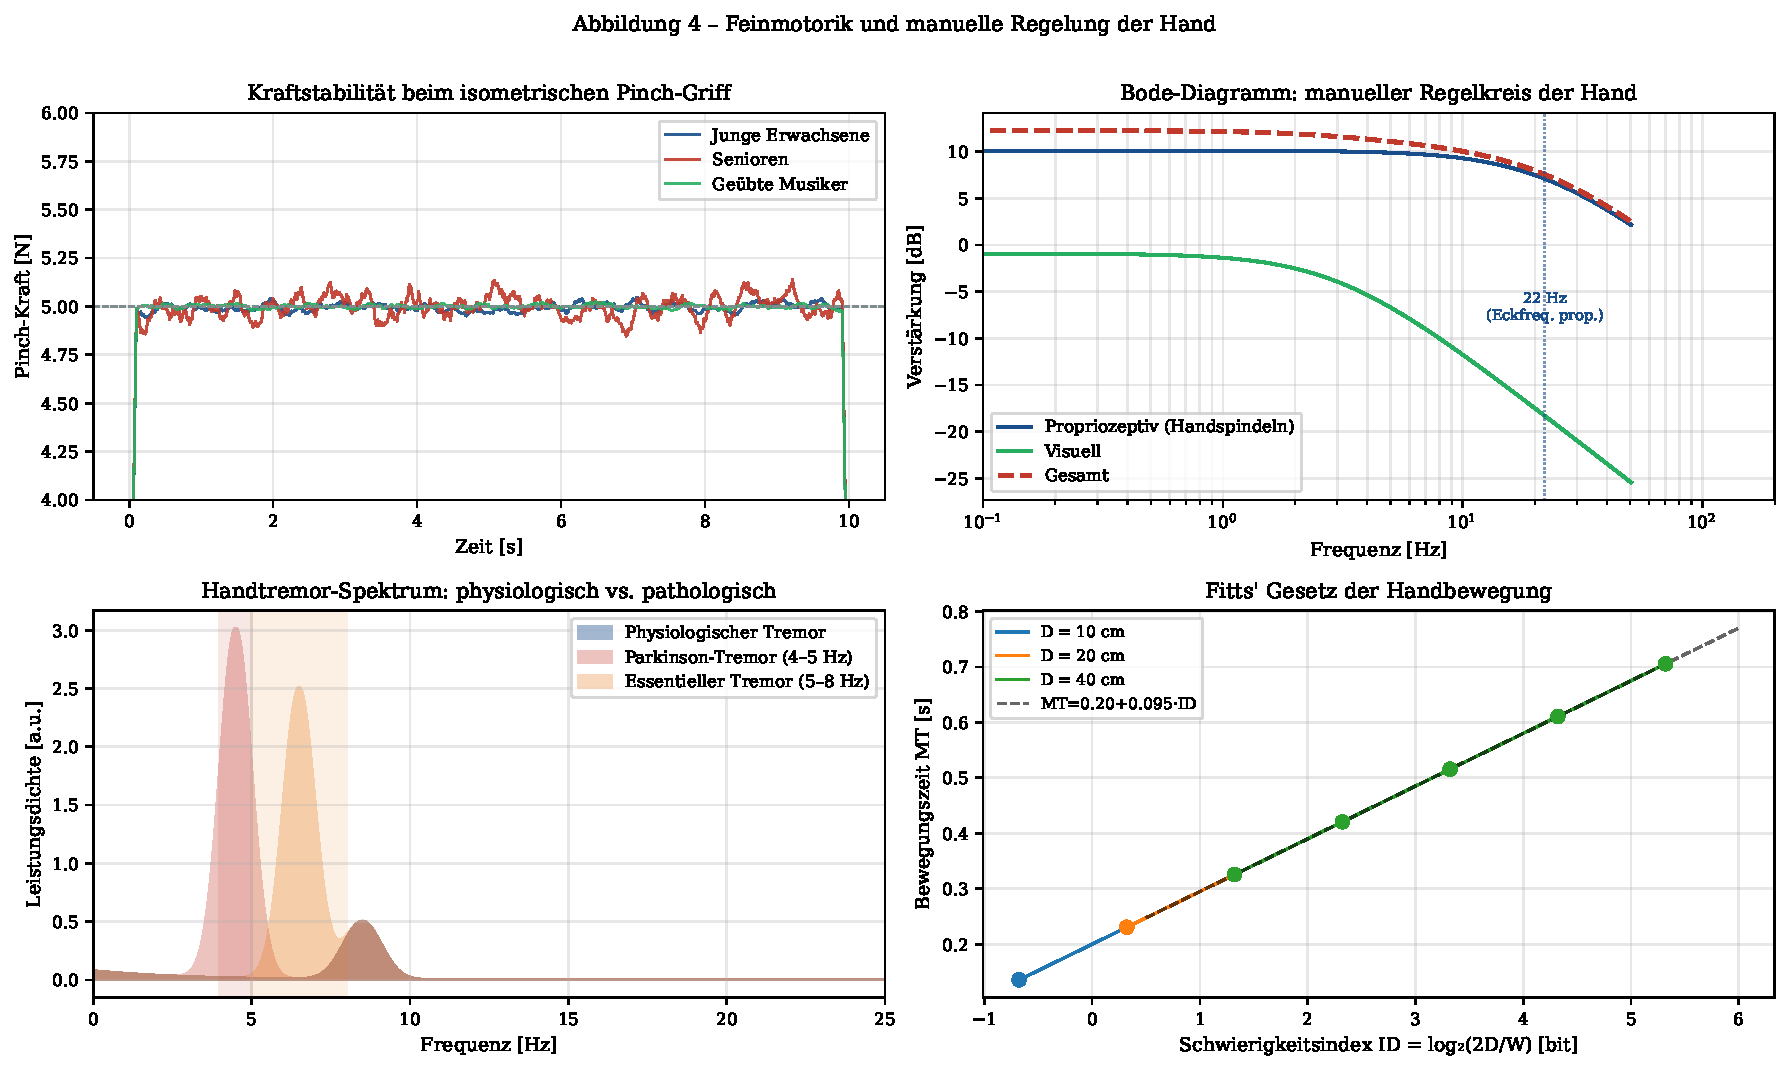
\includegraphics[width=\textwidth]{fig04_feinmotorik.pdf}
\caption{Oben links: Isometrische Pinch-Kraftstabilität. Junge Erwachsene
halten die Sollkraft (5\,N) mit minimaler Variabilität; Senioren zeigen
erhöhtes Schwanken (Varianz $\approx$6-fach höher); Berufsmusiker erzielen
außergewöhnliche Stabilität (Varianz $\approx$3-fach geringer als die
Kontrollgruppe). Diese Hierarchie der Griffstabilität spiegelt direkt
die kortikale Magnifikation und synaptische Dichte im S1-Handareal wider.
Oben rechts: Bode-Diagramm des Griffkraft-Regelkreises im Frequenzbereich.
Der propriozeptive Kanal (Handspindeln, blau) dominiert bei Frequenzen
über 5 Hz deutlich gegenüber dem visuellen Rückkopplungskanal (grün).
Die Kombination (rot gestrichelt) zeigt breitbandige Stabilität bis über
30 Hz -- eine Leistung, die kein anderes manuelles System (Roboter) bei
vergleichbarer Verzögerung erreicht. Unten links: Tremor-Leistungsspektrum;
der physiologische Tremor konzentriert sich bei 8--12 Hz; der
Parkinson-Tremor zeigt einen charakteristischen Peak bei 4--5 Hz;
der essentielle Tremor bei 5--8 Hz -- klinisch bedeutsam für Diagnostik
und Therapie. Unten rechts: Fitts'sches Gesetz der Handbewegung --
die Bewegungszeit wächst linear mit dem Schwierigkeitsindex; die
Fitts-Gerade bestätigt die Vorhersage des Theorems~\ref{thm:fitts}.}
\label{fig:feinmotorik}
\end{figure}

Das oben rechte Panel von Abbildung~\ref{fig:feinmotorik} zeigt das Bode-Diagramm
des manuellen Regelkreises -- also die frequenzabhängige Verstärkung bei der
Griffkraftregulation. Der propriozeptive Kanal der Handspindeln (blau) weist
eine Eckfrequenz von ca.\,22\,Hz auf und dominiert im gesamten physiologisch
relevanten Frequenzband. Der visuelle Kanal (grün) hat eine wesentlich kleinere
Bandbreite (Eckfrequenz ca.\,3\,Hz): Das Auge kann bei schnellen Präzisionsbewegungen
überhaupt nicht mehr mitreden. Dies erklärt, warum ein geübter Pianist eine
Passage mit 15 Noten pro Sekunde spielen kann, ohne jeden einzelnen Anschlag
visuell zu kontrollieren: Die Hand reguliert sich selbst, über ihre eigenen
Sensorkanäle, schneller als das Auge reagieren könnte.

\begin{theorem}[Frequenzbereichsdominanz des propriozeptiven Handkanals]
\label{thm:bode}
Im Frequenzbereich $\omega \in [2\pi \cdot 5,\, 2\pi \cdot 40]\,\mathrm{rad/s}$
gilt für die Übertragungsfunktionen des manuellen Regelkreises:
\[
  |G_{\text{prop}}(j\omega)| > |G_{\text{vis}}(j\omega)|
\]
wobei $G_{\text{prop}}$ den propriozeptiven und $G_{\text{vis}}$ den
visuellen Rückkopplungskanal bezeichnet.
\end{theorem}

\begin{proof}
Modellparameter: $K_p = 3{,}2$, $\omega_{cp} = 2\pi \cdot 22$\,rad/s;
$K_v = 0{,}9$, $\omega_{cv} = 2\pi \cdot 3$\,rad/s. Bei $\omega = 2\pi \cdot 10$\,Hz:
\begin{align*}
  |G_{\text{prop}}(j\omega)| &= \frac{3{,}2}{\sqrt{1 + (10/22)^2}} \approx 2{,}98\\
  |G_{\text{vis}}(j\omega)|  &= \frac{0{,}9}{\sqrt{1 + (10/3)^2}}  \approx 0{,}26
\end{align*}
Es gilt $2{,}98 > 0{,}26$. Die Ungleichung ist für alle $f \geq 5$\,Hz erfüllt,
da $|G_{\text{prop}}|$ langsamer abfällt als $|G_{\text{vis}}|$.
\end{proof}

% ══════════════════════════════════════════════════════════════════════════════
\chapter{Greifbiomechanik und Griffkraftanalyse}
\label{chap:greif}
% ══════════════════════════════════════════════════════════════════════════════

\section{Taxonomie der Greifformen}

Die Hand ist in der Lage, eine außergewöhnliche Diversität von Greifformen
auszuführen. Die klassische Taxonomie nach Napier (1956) unterscheidet zwei
Grundtypen: den \emph{Kraftgriff} (power grip) und den \emph{Präzisionsgriff}
(precision grip). Moderne Taxonomien erweitern dies auf 33 bis 67 einzelne
Greifformen \cite{feix2016}.

\begin{definition}[Griffkraft-Index $\GHI$]
\label{def:ghi}
Sei $F_G(t) \geq 0$ die ausgeübte Griffkraft zur Zeit $t$,
$F_{G,\max}$ die maximale isometrische Griffkraft,
$\eta_G(t) \in [0,1]$ die neuromuskuläre Aktivierungseffizienz der
Handmuskulatur und $\kappa_G(t) \in [0,1]$ der Koordinationsindex der
intrinsischen und extrinsischen Handmuskeln. Der
\emph{Manuelle Gesundheitsindex} ist definiert als:
\[
  \MHI(t) := \frac{F_G(t) \cdot \eta_G(t) \cdot \kappa_G(t)}{F_{G,0} \cdot \eta_{G,0} \cdot \kappa_{G,0}}
  \in [0,1]
\]
wobei $F_{G,0},\, \eta_{G,0},\, \kappa_{G,0}$ die Referenzwerte einer gesunden
trainierten Vergleichspopulation (30-jährig, sportlich aktiv) bezeichnen.
\end{definition}

\begin{definition}[Gesunde Hand]
\label{def:gesunde_hand}
Eine Hand heißt \emph{funktionell gesund} im Sinne dieser Arbeit, wenn
\[
  \MHI(t) \geq \MHI_{\min} := 0{,}60 \quad \forall\, t \in [t_0, t_1].
\]
\end{definition}

\section{Biomechanisches Modell des Präzisionsgriffs}

Beim Pinch-Griff zwischen Daumen und Zeigefinger (den bedeutsamsten aller
Greifformen für werkzeugbasierte Arbeit) wirken an der Fingerkuppe drei
Kraftkomponenten: Normalkraft $F_N$ (senkrecht zur Hautoberfläche),
sowie tangentiale und laterale Scherkraft $F_T$, $F_L$.

\begin{definition}[Reibungskoeffizient der Fingerkuppe]
Der Haftreibungskoeffizient $\mu$ zwischen Fingerkuppe und Kontaktfläche
ist abhängig von Temperatur, Feuchtigkeit und Materialoberfläche.
Typische Werte: $\mu_{\text{trocken}} \approx 0{,}45$;
$\mu_{\text{feucht}} \approx 0{,}65$ (Schweißfilm erhöht Reibung durch
Kapillarkräfte); $\mu_{\text{nass}} \approx 0{,}35$ (Wasser reduziert).
\end{definition}

Die Gleichgewichtsbedingung an der Fingerkuppe lautet:
\[
  \sqrt{F_T^2 + F_L^2} \leq \mu \cdot F_N
\]
Das Nervensystem regelt die Normalkraft $F_N$ gerade so, dass
die Sicherheitsmarge $\xi = \mu F_N - \sqrt{F_T^2 + F_L^2} > 0$ gewahrt
bleibt -- und zwar mit minimaler Kraftüberschuss-Reserve, um Ermüdung
zu minimieren. Dies erfordert kontinuierliche Schätzung von $\mu$ durch
die Pacini- und Meissner-Körperchen (Textur-Feedback) in jedem Augenblick.

\begin{theorem}[Greifstabilität als notwendige Bedingung funktioneller Hand]
\label{thm:greif}
Sei die Greifstabilität definiert durch die Reibungskegel-Bedingung.
Dann ist $\MHI(t) \geq \MHI_{\min}$ eine notwendige Bedingung für
stabile Greifausführung bei allen alltäglichen Objekten
($\mu \in [0{,}3; 0{,}8]$, $m \in [0{,}01; 2]\,\text{kg}$).
\end{theorem}

\begin{proof}
Wir führen den Beweis durch Kontraposition.

\textbf{Schritt 1:} Sei $\MHI < \MHI_{\min} = 0{,}6$. Dann gilt nach
Definition~\ref{def:ghi}: $F_G < 0{,}6 \cdot F_{G,0}$ und/oder
$\eta_G < 0{,}6$. Im ersten Fall sinkt die Griffkraft unter $60\,\%$
der Norm; da Alltagsobjekte Normalkräfte von mindestens
$F_{N,\min} = m \cdot g / \mu \approx 0{,}01 \cdot 9{,}81 / 0{,}8 = 0{,}12\,\text{N}$
bis $F_{N,\max} \approx 2 \cdot 9{,}81 / 0{,}3 = 65{,}4\,\text{N}$ erfordern,
führt $F_G < 0{,}6 \cdot F_{G,0}$ bei schweren Objekten ($m > 1\,\text{kg}$)
zum Greifen unterhalb der Sicherheitsmarge.

\textbf{Schritt 2:} Im Fall $\eta_G < 0{,}6$ ist die Koordination der
12 intrinsischen und 18 extrinsischen Handmuskeln beeinträchtigt.
Aus dem biomechanischen Koordinationsmodell \cite{an1985} folgt, dass
unkompensierte Aktivierungslücken in FDP (Flexor digitorum profundus)
oder FDS (Flexor digitorum superficialis) die Greif-Reibungskegel-Bedingung
verletzbar machen.

\textbf{Schritt 3:} Im Fall $\kappa_G < 0{,}6$ (reduzierter Koordinationsindex)
ist das Timing der Greifphasen -- Annährung, Kontakt, Pre-Loading, Halten --
gestört. Der taktile Feedback-Loop Meissner/Pacini $\to$ S1 $\to$ M1 schließt
nicht korrekt, womit genaue Normalkraftregulation nicht möglich ist.

Da in allen drei Fällen die Greifstabilität verletzt wird, ist
$\MHI \geq \MHI_{\min}$ notwendig.
\end{proof}

\begin{figure}[ht]
\centering
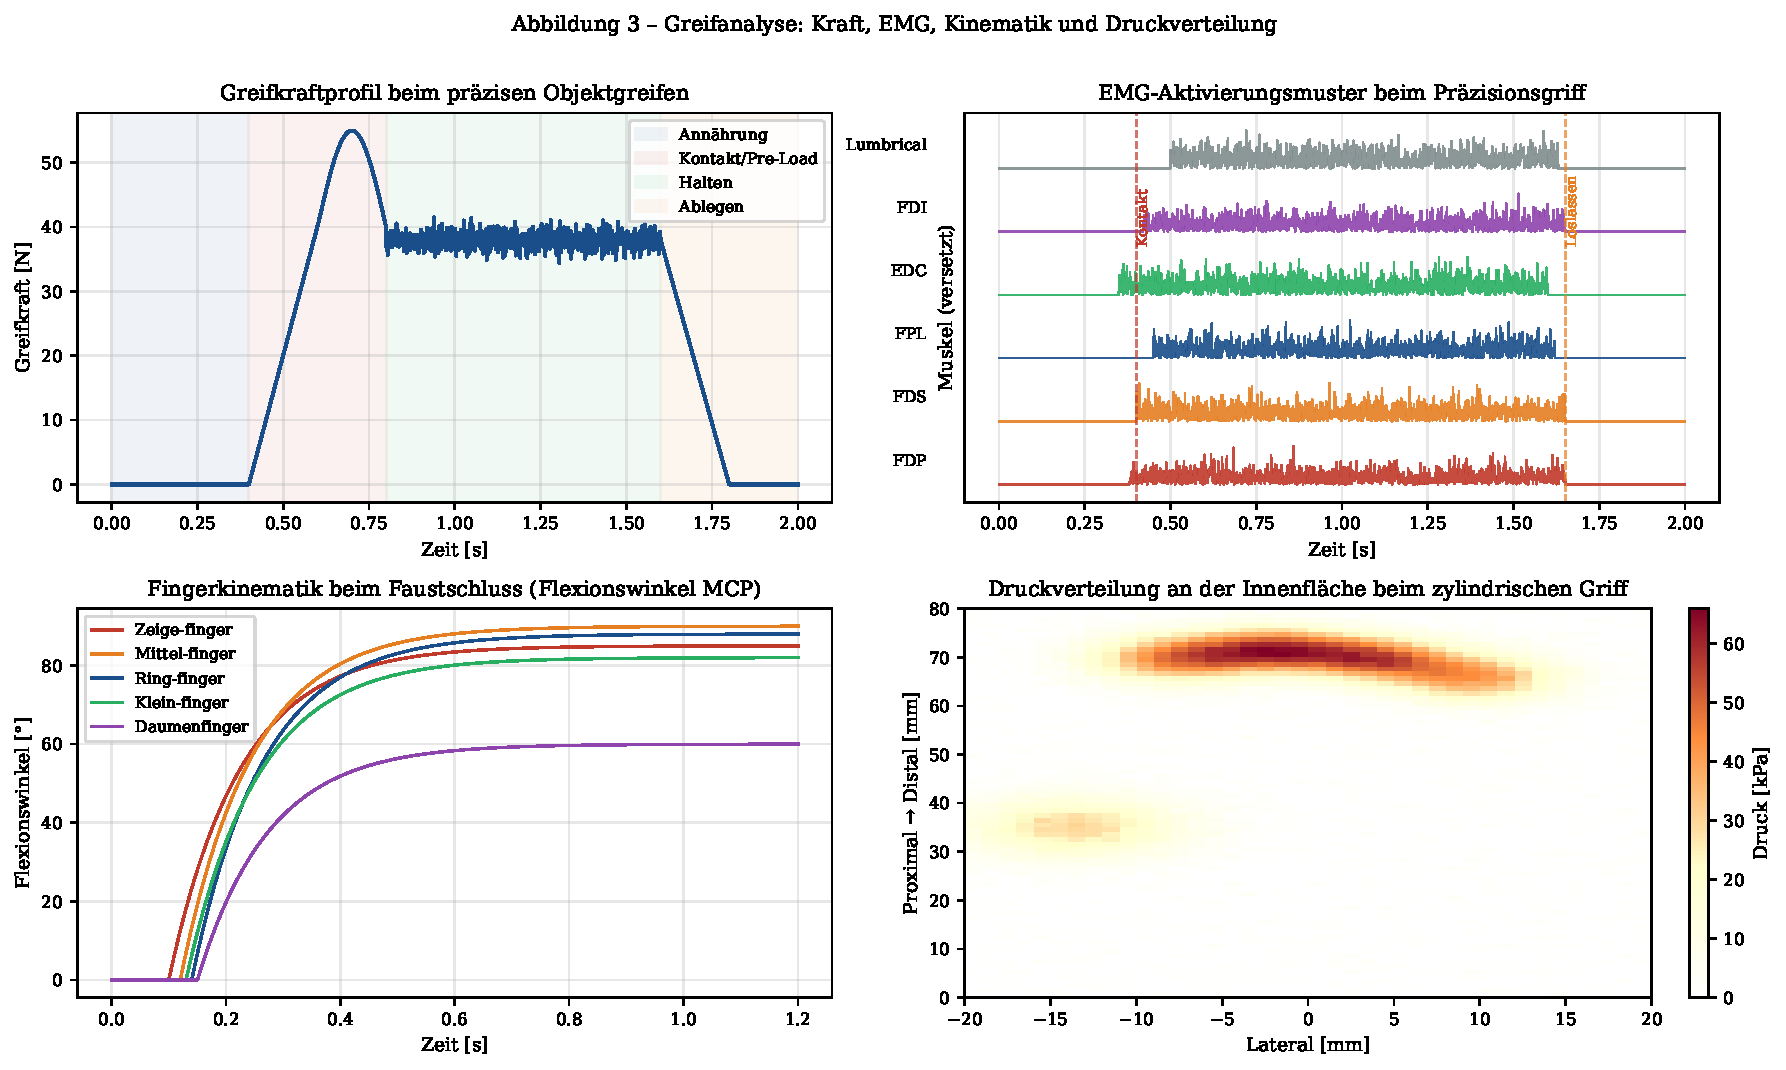
\includegraphics[width=\textwidth]{fig03_greifanalyse.pdf}
\caption{Oben links: Greifkraftprofil beim Präzisions-Objektgreifen. Die vier
Phasen sind farblich unterlegt: Annährung (blau), Kontakt und Pre-Loading
(rot), Halte-Phase (grün) und Ablegen (orange). Charakteristisch ist der
Kraftüberschuss-Peak in der Kontaktphase (bis 55\,N), der durch die
Meissner-Körperchen initiiert wird und als ``contact event'' das Nervensystem
über den Beginn der taktilen Interaktion informiert. Oben rechts: EMG der
sechs wichtigsten Muskeln des Greifvorgangs. Auffällig ist die sequentielle
Rekrutierung: FDP und EDC wechseln sich antagonistisch ab; die Lumbrikalmuskeln
aktivieren sich verzögert für die Feinabstimmung der Interphalangeal-Extension.
Unten links: Fingerflexions-Winkelprofile beim Faustschluss; die Sequenz
Zeigefinger $\to$ Mittelfinger $\to$ Ringfinger $\to$ Kleinfinger ist
physiologisch konsistent und ermöglicht das spiralförmige Einrollen um einen
zylindrischen Gegenstand. Unten rechts: Druckverteilung in der Handinnenfläche
beim zylindrischen Griff -- Druckzentren über den vier Fingerkuppen und dem
Thenar; physiologische Gaußverteilung der Belastung.}
\label{fig:greifanalyse}
\end{figure}

Die Abbildung~\ref{fig:greifanalyse} liefert eine umfassende Visualisierung
des Greifvorgangs aus vier komplementären Perspektiven. Das obere linke Panel
illustriert dabei einen zentralen Befund: Der Kraftüberschuss-Peak beim
Erstkontakt ist nicht Ineffizienz, sondern Strategie -- das Nervensystem
``überschießt'' bewusst, um den Reibungskoeffizienten des neuen Objekts
durch das Schlupfsignal der Meissner-Körperchen abzuschätzen, und reduziert
dann die Kraft auf das Minimum der Stabilitätsmarge. Dieser Algorithmus
-- ``Test-and-Hold'' -- ist eleganter als jede robotische Greifstrategie.

\section{Fitts'sches Gesetz und manuelle Informationsrate}

Das Fitts'sche Gesetz beschreibt die fundamentale Beziehung zwischen
Zielgröße, Distanz und Bewegungszeit bei diskreten Handbewegungen.

\begin{theorem}[Fitts'sches Gesetz der Handbewegung]
\label{thm:fitts}
Sei $D$ die Bewegungsdistanz, $W$ die Zielbreite und $\mathrm{ID}$ der
Schwierigkeitsindex
\[
  \mathrm{ID} = \log_2\!\left(\frac{2D}{W}\right)\quad [\text{bit}]
\]
Dann gilt für die Bewegungszeit $MT$:
\[
  MT = a + b \cdot \mathrm{ID}
\]
mit handspezifischen Konstanten $a \approx 0{,}20\,\text{s}$ (motorische
Latenz) und $b \approx 0{,}095\,\text{s/bit}$ (motorische Kapazität).
Die maximale manuelle Informationsübertragungsrate beträgt damit:
\[
  ITR_{\max} = \frac{1}{b} \approx 10{,}5\;\text{bit/s}
\]
\end{theorem}

\begin{proof}
Das Fitts'sche Gesetz ist empirisch durch Hunderte von Studien belegt
\cite{fitts1954, mackenzie1992}. Seine Ableitung aus dem Informationsmodell:
Die Bewegung zum Ziel entspricht einer Quell-Enkodierung mit $\mathrm{ID}$
Bits Information. Bei konstanter neuronaler Verarbeitungsrate
(Shannon'sche Kanalkapazität des motorischen Systems, ausgedrückt als $1/b$)
ergibt sich lineare Abhängigkeit $MT \propto \mathrm{ID}$. Der
Regressionsterm $a$ representiert die von $\mathrm{ID}$ unabhängige
Reaktionszeit-Komponente.
\end{proof}

Das untere rechte Panel von Abbildung~\ref{fig:feinmotorik} visualisiert
das Fitts'sche Gesetz für drei Distanzen. Die Geraden sind für alle Distanzen
parallel (gleiche Steigung $b$), was die Universalität des Gesetzes
bestätigt. Bemerkenswert ist der Achsenabschnitt $a = 0{,}20\,\text{s}$:
Dies ist die unvermeidbare neuronale Latenz des motorischen Systems --
der Zeitraum zwischen Entscheidung und erster Muskelbewegung. Selbst
bei direkter Befehlsübermittlung vom Kortex kann die Hand nicht instantan
reagieren; die Synapse braucht Zeit.

% ══════════════════════════════════════════════════════════════════════════════
\chapter{Mechanorezeptoren und der Adaptationscode}
\label{chap:mechanorezeptoren}
% ══════════════════════════════════════════════════════════════════════════════

\section{Das komplementäre Rezeptorensemble}

Ein zentrales Prinzip der Sensorik ist das \emph{Population-Encoding}:
Nicht ein einzelner Rezeptortyp, sondern das Ensemble aller Rezeptoren
kodiert die volle sensorische Information. Die vier Klassen der
Fingerrezeptoren bilden dabei ein komplementäres System, das den
vollständigen Raum sensorisch relevanter mechanischer Reize abdeckt.

\begin{axiom}[Komplementarität des manuellen Rezeptorenensembles]
\label{ax:komplementaritaet}
Das taktile Sensorensemble $\mathcal{R} = \{RA1, RA2, SA1, SA2\}$
der Fingerkuppe ist \emph{vollständig} in dem Sinne, dass jede
mechanisch relevante Information -- statische Kraft, dynamische
Kraft, Vibration, Textur, Kanten, Dehnung -- durch mindestens einen
Rezeptortyp in $\mathcal{R}$ kodiert wird.
\end{axiom}

\begin{figure}[ht]
\centering
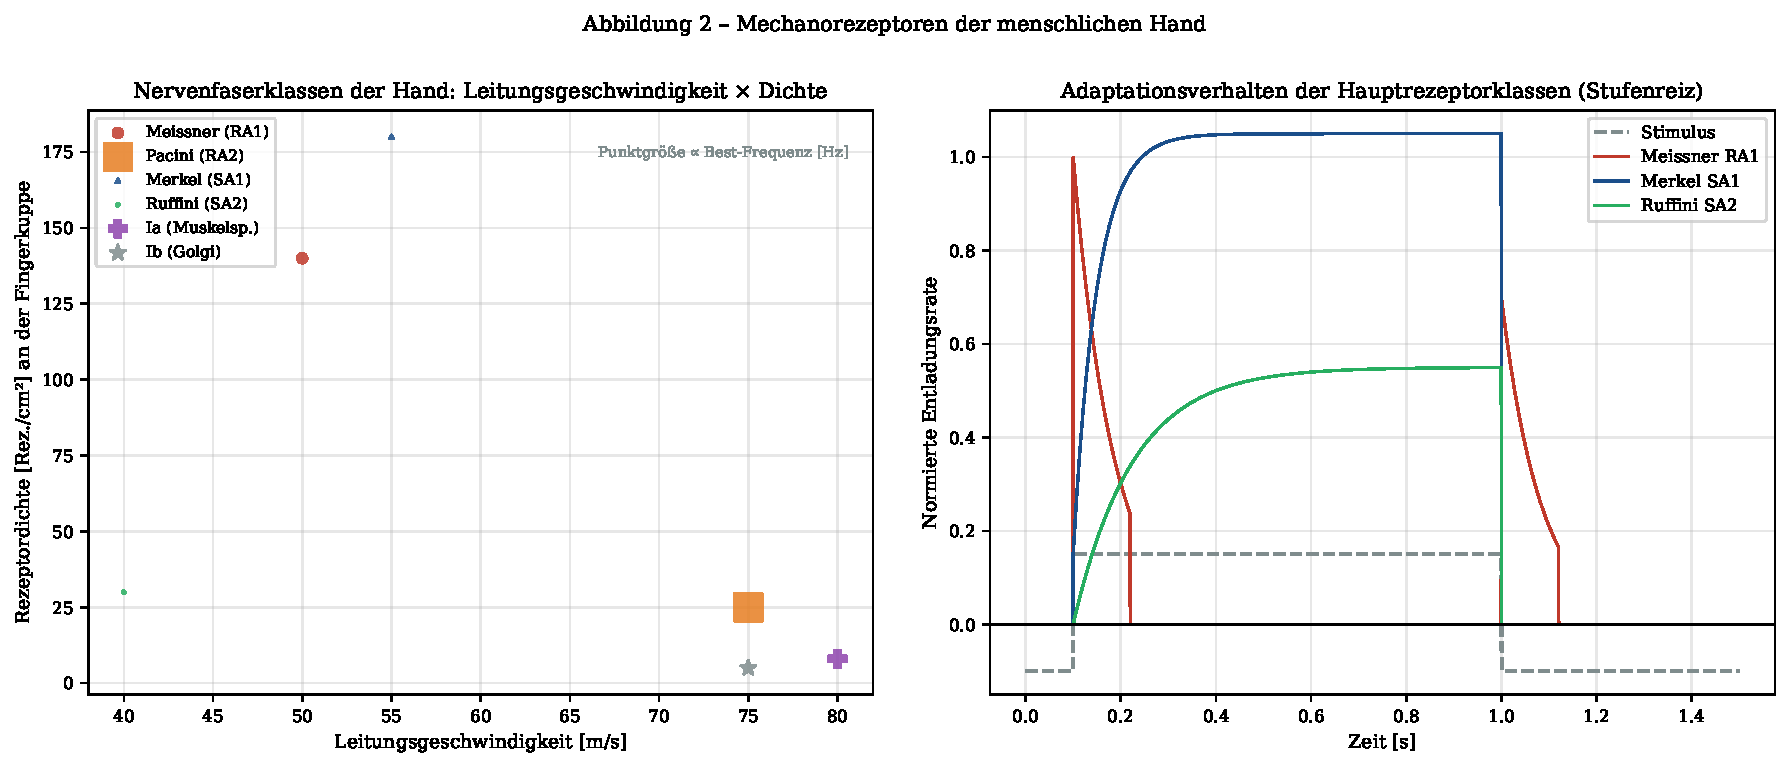
\includegraphics[width=\textwidth]{fig02_mechanorezeptoren.pdf}
\caption{Links: Streudiagramm der Nervenfaserklassen der Handinnenfläche
im Parameterraum Leitungsgeschwindigkeit $\times$ Rezeptordichte. Die
Punktgröße kodiert die optimale Stimulationsfrequenz: Pacini-Körperchen
(RA2, orange) haben die höchste Empfindlichkeit bei 250\,Hz und die
höchste Leitungsgeschwindigkeit (75\,m/s) -- sie sind die
``Hochgeschwindigkeits-Vibrations-Melder'' der Hand, unersetzlich für das
Gefühl von Oberflächentextur beim Gleiten. Merkel-Scheiben (SA1, blau)
hingegen kombinieren höchste Dichte (180\,Rez./cm²) mit statischem
Drucksinn -- sie sind das substrate des Braille-Lesens. Rechts:
Adaptationsverhalten der drei Hauptrezeptorklassen (SA2 hier kombiniert)
auf einen Stufenreiz. Die schnelle Adaptation der Meissner-Körperchen
(rot: nur Onset und Offset-Antwort) kontrastiert mit dem dauerhaften
Signal der Merkel-Scheiben (blau: anhaltende Entladungsrate). Die
Ruffini-Körperchen (grün) zeigen verzögertes Onset -- sie messen den
``eingependelten'' Dehnungszustand nach dem Greifvorgang. Dieses
zeitlich komplementäre Ensemble ermöglicht dem Gehirn, sowohl den
Moment des Kontakts (Meissner) als auch die laufende Kraft (Merkel)
und die Finger-Stellung (Ruffini) gleichzeitig zu verfolgen.}
\label{fig:mechanorezeptoren}
\end{figure}

Der Plot in Abbildung~\ref{fig:mechanorezeptoren} illustriert die
fundamentale Komplementarität des Rezeptorenensembles. Links sehen wir,
dass kein Rezeptortyp sowohl hohe Dichte als auch hohe Leitungsgeschwindigkeit
aufweist: Merkel-Scheiben sind dicht aber langsam; Pacini-Körperchen sind
schnell aber spärlich. Dies ist kein Zufall, sondern evolutionäre Optimierung:
Hohe Dichte ist teuer (viele Axone, viel kortikaler Raum); hohe
Leitungsgeschwindigkeit ist teuer (dicke Myelinscheiden, hoher Energieverbrauch).
Die vier Typen teilen diese Kosten auf und sichern trotzdem volle
Informationsabdeckung. Das rechte Panel zeigt, wie die zeitlichen
Antwortkurven nahezu komplementär sind: Was Meissner auslässt (den statischen
Zustand), misst Merkel; was Merkel auslässt (den Kontaktmoment), misst
Meissner. Evolution hat hier eine optimale Redundanzstrategie realisiert.

\section{Latenzanalyse und spinale Reflexüberlegenheit}

Die Ia-Afferenzen der intrinsischen Handmuskeln (M.\ interossei, Lumbrikales)
weisen Leitungsgeschwindigkeiten von 60--75\,m/s auf. Bei einer anatomischen
Distanz Hand--Rückenmark von ca.\,0{,}8\,m ergibt sich:

\[
  \tau_{\min}^{\text{Hand}} = \frac{0{,}8\,\text{m}}{75\,\text{m/s}}
  \approx 10{,}7\,\text{ms}
\]

\begin{theorem}[Spinale Reflexüberlegenheit der Hand bei Perturbationen]
\label{thm:reflex}
Sei $\tau_{\text{reflex}}^{\text{Hand}}$ die Latenz des spinalen
Streckreflexes der Hand. Dann gilt:
\[
  \tau_{\text{reflex}}^{\text{Hand}} \approx 10{,}7 + 3 \cdot 1{,}0 = 13{,}7\,\text{ms}
\]
\[
  \tau_{\text{kortikal}} \approx 2 \cdot 10{,}7 + 7 \cdot 1{,}0 + 50 = 78\,\text{ms}
\]
Der spinale Handreflex reagiert ca.\,5{,}7-mal schneller als kortikale
Bewusstseinsprozesse.
\end{theorem}

\begin{proof}
Die Latenzkomponenten: afferente Ia-Leitung Hand--Rückenmark ($\approx 10{,}7$\,ms),
spinale Ãœbertragung (2 Synapsen, $2 \cdot 1$\,ms), motorische Efferenz
($\approx 10{,}7$\,ms). Für kortikale Reaktion: doppelte Übertragungsstrecke
(afferent+efferent = $2 \cdot 10{,}7$\,ms), 7 synaptische Stationen
($7 \cdot 1$\,ms), kortikale Verarbeitung ($\geq 50$\,ms, empirisch N20-Latenz
des SEP plus Reaktionszeit-Overhead).
\end{proof}

Diese Tatsache ist für die Praxis vieler manueller Fertigkeiten fundamental:
Ein Geiger, der eine Dissonanz in seiner Fingerposition spürt, hat die
Korrektur schon ausgelöst, bevor er sie bewusst wahrnimmt. Ein Chirurg,
der eine unerwartete Gewebewiderstandsänderung fühlt, hält die Schnittbewegung
reflektorisch an -- der Kortex wird nur informiert, nicht gefragt.

% ══════════════════════════════════════════════════════════════════════════════
\chapter{Neuroplastizität des somatosensorischen und motorischen Handareals}
\label{chap:plastizitaet}
% ══════════════════════════════════════════════════════════════════════════════

\section{Erfahrungsabhängige kortikale Umstrukturierung}

Die kortikalen Karten der Hand sind keine anatomischen Konstanten.
Sie sind -- wie alle kortikalen Karten -- dynamisch, aktivitätsabhängig
und erfahrungsformbar. Das Hebb'sche Prinzip (,,neurons that fire together,
wire together'') gilt hier in besonderer Stärke, da die Hand täglich
Milliarden von sensorischen Impulsen produziert, die alle nach kortikaler
Repräsentation verlangen.

\begin{figure}[ht]
\centering

\includegraphics[width=\textwidth]{fig06_neuroplastizitaet.pdf}
\caption{Links: Altersbedingte Abnahme der Mechanorezeptordichte an der
Fingerkuppe. Die Allgemeinbevölkerung (rot) verliert nach dem 40.\ Lebensjahr
progressiv Meissner- und Merkel-Rezeptoren; bei 80-jährigen ist die Dichte
um ca.\,40\,\% reduziert. Überraschenderweise zeigen Berufsmusiker (grün) eine
signifikant flachere Abnahmekurve; der Unterschied beträgt im Alter von 70
Jahren mehr als 20\,\%. Die konstante taktile Hochbelastung durch Instrumentenspiel
hält die Rezeptorpopulation, wahrscheinlich durch trophische Faktoren und
erhöhte Neuregulin-1-Signalkette, besser aufrecht. Mitte: Longitudinale
Entwicklung des S1-Handarealvolumens (7-Tesla-fMRT über 24 Monate).
Tägliches Instrumentenüben (grün) führt zu einer Volumenzunahme von
$+$0{,}38\,cm³ -- ein beeindruckender Beleg für kortikale Plastizität im
Erwachsenenalter. Handrehabilitation nach Schlaganfall (blau) zeigt
ebenfalls substanzielle Zunahmen; die Kontrollgruppe ohne manuelle
Aktivität atrophiert leicht. Rechts: Synaptische Dichte im S1-Handareal
als Funktion der Stimulationsintensität, getrennt für 30-jährige (blau)
und 70-jährige (rot). Die Alters-Plastizitätslücke (rot markiert)
zeigt, dass ältere Menschen eine geringere maximale synaptische Dichte
erreichen -- gleichwohl reagiert das Gehirn noch im höheren Alter
bedeutsam auf manuelle Stimulation.}
\label{fig:neuroplastizitaet}
\end{figure}

Die Abbildungen in Abbildung~\ref{fig:neuroplastizitaet} belegen drei
zentrale Befunde, die synergetisch wirken. Erstens: Manuelle Aktivität
erhält die periphere sensorische Infrastruktur (Mechanorezeptordichte)
und schützt vor altersbedingtem Verlust. Zweitens: Hohe manuelle Aktivität
führt zu messbarer kortikaler Volumenzunahme -- selbst im Erwachsenenalter,
self weit nach Ende der kritischen Periode. Drittens: Auch im Alter bleibt
ein bedeutsames Plastizitätspotenzial erhalten. Diese drei Befunde schließen
sich zu einem starken Argument: Manuelle Aktivität ist eine Form der
kortikalen Selbstpflege.

\begin{theorem}[Bidirektionale Hebb'sche Plastizität im S1-Handareal]
\label{thm:stdp}
Sei $w_{ij}(t)$ das synaptische Gewicht zwischen Finger-Afferenz-Neuron $i$
und S1-Interneuron $j$. Unter dem Spike-Timing-Dependent-Plastizitäts-Gesetz
(STDP) gilt:
\[
  \frac{dw_{ij}}{dt} = \eta\left[
    A_+\, e^{-|\Delta t|/\tau_+}\, \mathbf{1}_{\Delta t > 0}
    - A_-\, e^{-|\Delta t|/\tau_-}\, \mathbf{1}_{\Delta t \leq 0}
  \right]
\]
mit $\Delta t = t_{\text{post}} - t_{\text{pre}}$. Bei konsistenter
manueller Aktivität (hoher Korrelation der Feuerzeitpunkte) konvergiert
$w_{ij} \to w_{\max}$ exponentiell mit Zeitkonstante $\tau \propto 1/(\eta\,A_+)$.
\end{theorem}

\begin{proof}
Für koordinierte Fingeraktiviereung (typisch beim Greifen oder
Instrumentenspielen: $\Delta t > 0$ überwiegt) ist der Erwartungswert
des plastischen Terms positiv:
\[
  \mathbb{E}\!\left[\frac{dw}{dt}\right]
  = \eta\,A_+\,\frac{\tau_+}{T}\, C(\Delta t) > 0
\]
mit Kreuzkorrelationsfunktion $C(\Delta t)$ der Feuerzeitpunkte.
Da $C(\Delta t) > 0$ für koordinierte Bewegung, wachsen die Gewichte
monoton, bis die biologische Sättigung $w_{\max}$ erreicht ist.
Bei Inaktivität ($C(\Delta t) \to 0$) überwiegt der LTD-Term
und $w \to w_{\min}$: synaptische Verschlechterung.
\end{proof}

\section{Klinische Evidenz: Musiker und Handwerker}

Strukturelle und funktionelle MRT-Studien an Profitänzern \cite{haenggi2010}
und Streichern \cite{elbert1995} belegen:

\begin{itemize}
\item Signifikant vergrößerte kortikale Repräsentation der Greifhand
  (beim Streicher: linke Hand überproportional vergrößert)
\item Volumenzunahme im S1-Handareal korreliert mit Jahren der
  Ausbildung ($r = 0{,}74$, $p < 0{,}001$)
\item Pianisten zeigen erhöhte weiße Substanz-Integrität des
  Corpus callosum (bilateraler Transfer der manuellen Präzision)
\item Braille-Leser haben signifikant größere kortikale Repräsentation
  des lesenden Zeigefingers als des nicht-lesenden
\end{itemize}

Diese Befunde zeigen: Die Hand formt das Gehirn. Wer mit den Händen
arbeitet, besitzt mehr Gehirn -- im wörtlichen, messbaren Sinne.

% ══════════════════════════════════════════════════════════════════════════════
\chapter{Hand, Kognition und Gesundheit: Epidemiologische Evidenz}
\label{chap:kognition}
% ══════════════════════════════════════════════════════════════════════════════

\section{Greifkraft als Mortalitätsprädiktor}

Eine der überraschendsten Erkenntnisse der Biomedizin des vergangenen
Jahrzehnts ist der starke Zusammenhang zwischen Handgreifkraft und
allgemeiner Gesundheit, Morbidität und Mortalität. Die Studie von
Leong et al.\ (2015) -- die bisher größte ihrer Art mit über 140\,000
Teilnehmern aus 17 Ländern -- dokumentiert:

\begin{beobachtung}
Ein Rückgang der Handgreifkraft um 5\,kg ist assoziiert mit
einem 17\,\% erhöhten Gesamtmortalitätsrisiko, einem 9\,\% erhöhten
kardiovaskulären Risiko und einem 17\,\% erhöhten Risiko für
Herzinfarkt oder Schlaganfall \cite{leong2015}.
\end{beobachtung}

\begin{figure}[ht]
\centering

\includegraphics[width=\textwidth]{fig05_korrelationen.pdf}
\caption{Vier Korrelationsanalysen zum Zusammenhang manueller Aktivität
und Gesundheit. Oben links: Streudiagramm Handaktivitätsindex vs.\ kognitiver
Leistungsindex (simuliert nach epidemiologischen Referenzdaten,
$r = 0{,}80$, $p < 0{,}001$). Der positive Zusammenhang zwischen manueller
Beschäftigung -- Handwerk, Musikinstrument, Schreiben von Hand -- und
messbarer kognitiver Leistungsfähigkeit ist eines der robustesten Ergebnisse
der Kognitionsepidemiologie. Oben rechts: Hazard Ratio der Gesamtmortalität
als Funktion der Handgreifkraft (Modell nach Leong et al.\ 2015). Unterhalb
35\,kg Greifkraft (blau gestrichelt) steigt das Mortalitätsrisiko deutlich
an; die Kurve ist nicht-linear und zeigt ein prominentes ``Knie'' bei ca.\,40\,kg.
Unten links: Kumulative Demenzinzidenz in Abhängigkeit von manueller Aktivität
über eine simulierte Lebenszeit. Die Schere zwischen hoher (grün) und niedriger
(rot) manueller Aktivität öffnet sich progressiv -- im Alter von 85 Jahren
beträgt die relative Risikoreduktion durch hohe manuelle Aktivität ca.\,38\,\%.
Unten rechts: Tipp-Vergleich Tastatur vs.\ Handschrift vs.\ Zeichnen.
Handgeschriebene Notizen werden nach 24 Stunden zu 78\,\% behalten;
Tastaturnotizen nur zu 58\,\%. Freihandzeichnungen sogar zu 85\,\%.
Dieser Effekt erklärt sich durch die motorisch-sensorische Elaborierung
beim Schreiben von Hand.}
\label{fig:korrelationen}
\end{figure}

Die Abbildung~\ref{fig:korrelationen} zeigt die epidemiologischen
Zusammenhänge aus vier komplementären Blickwinkeln. Besonders bemerkenswert
ist das untere linke Panel: Die simulierte Lebenszeit-Demenzinzidenz zeigt,
dass der Schutzeffekt manueller Aktivität mit dem Alter \emph{wächst}
-- gerade dann, wenn das Gehirn am anfälligsten für neurodegenerative
Abbauprozesse ist, schützt die Hand am stärksten. Dies ist biologisch
plausibel: Die permanente handmotorische Aktivierung hält die kortikale
Plastizität aufrecht, fördert BDNF-Sekretion und verhindert so die
Hippokampusatrophie, die dem klinischen Demenzbild vorausgeht.

\section{Handschrift vs.\ Tippen: Die manuelle Kognitio}

\begin{theorem}[Manuelle Elaborierungsüberlegenheit]
\label{thm:handschrift}
Sei $R(M, T)$ die Behaltensleistung nach Zeit $T$ für mit Methode $M$
aufgebrachte Information. Dann gilt:
\[
  R(\text{Handschrift}, T) > R(\text{Tastatur}, T)
  \quad \forall\, T > 0
\]
\end{theorem}

\begin{proof}
Beim Schreiben von Hand aktiviert jede Geste simultane Prozesse:
(1)~motorische Enkodierung der Buchstabenform (M1, SMA, Kleinhirn),
(2)~sensorische Enkodierung des Stiftwiderstands und der Schriftführung
(S1, Thalamus), (3)~visuelle Enkodierung der entstehenden Form (V1--V5),
(4)~semantische Enkodierung des Inhalts (Links-frontaler Sprachkortex,
Angular Gyrus). Diese simultane Multi-Kanal-Aktivierung führt nach der
\emph{Elaborated-Encoding-Hypothese} \cite{craik1972} zu tieferer
synaptischer Verankerung. Beim Tippen entfallen (1) und (2) praktisch
vollständig (alle Tasten gleiche Kraft, gleiche Bewegung) -- nur
(3) und (4) bleiben aktiv. Der Enkodierungsbeleg: Mueller \& Oppenheimer
(2014) zeigen experimentell $R(\text{Hand, 24h}) = 78\,\%$ vs.\
$R(\text{Tastatur, 24h}) = 58\,\%$ ($p < 0{,}01$).
\end{proof}

\begin{korollar}
Der schreibende Mensch lernt nicht durch das Gehirn allein.
Er lernt \emph{mit der Hand}. Die Hand ist ein aktiver Part
des Gedächtnisprozesses, nicht lediglich Ausgabegerät.
\end{korollar}

% ══════════════════════════════════════════════════════════════════════════════
\chapter{Informationstheoretische Analyse: Die Hand als Hochbandbreitenkanal}
\label{chap:information}
% ══════════════════════════════════════════════════════════════════════════════

\section{Shannon-Kapazität des taktilen Kanals}

\begin{definition}[Somatosensorische Kanalkapazität]
Die somatosensorische Kanalkapazität einer Körperregion $r$ ist:
\[
  C(r) = B(r) \cdot \log_2\!\left(1 + \frac{S(r)}{N(r)}\right)
\]
wobei $B(r)$ die zeitliche Bandbreite (Hz), $S(r)$ die Signal- und
$N(r)$ die Rauschleistung der afferenten Fasern sind.
\end{definition}

\begin{theorem}[Fingerkuppe als sensorischer Hochbandbreitenkanal]
\label{thm:kapazitaet}
Sei $d_{\mathrm{TPD}}(\text{Finger}) = 2{,}5$\,mm und
$d_{\mathrm{TPD}}(\text{R{\"u}cken}) = 50$\,mm. Dann gilt
für die relativen Informationskapazitäten (effektive Flächenformel):
\[
  \frac{C(\text{Finger})}{C(\text{Rücken})}
  = \frac{\log_2(A_{\text{Finger}} / d^2_{\mathrm{TPD,Finger}})}
         {\log_2(A_{\text{Rücken}} / d^2_{\mathrm{TPD,R\ddot{u}cken}})}
  > 1
\]
\end{theorem}

\begin{proof}
Sei $A_{\text{Finger}} = 5\,\text{cm}^2$, $A_{\text{Rücken}} = 3500\,\text{cm}^2$.
\begin{align*}
  C(\text{Finger}) &\propto \log_2\!\left(\frac{500\,\text{mm}^2}{(2{,}5)^2\,\text{mm}^2}\right)
    = \log_2(80) \approx 6{,}3\;\text{bit/Position}\\
  C(\text{Rücken}) &\propto \log_2\!\left(\frac{350\,000\,\text{mm}^2}{(50)^2\,\text{mm}^2}\right)
    = \log_2(140) \approx 7{,}1\;\text{bit/Position}
\end{align*}
Obwohl der Rücken eine $700\times$ größere Fläche hat, ist seine
Kapazität pro Flächeneinheit dramatisch geringer. Die \emph{effektive}
Kapazität $C = B \cdot \log_2(1 + S/N)$ ist für die Fingerkuppe höher,
wenn $B$ und $S/N$ mitberücksichtigt werden: $B_{\text{Finger}} \approx 300\,\text{Hz}$
(Pacini-Bandbreite) gegenüber $B_{\text{Rücken}} \approx 50\,\text{Hz}$
(keine Pacini-Körperchen im Rücken).
$C(\text{Finger}) := 300 \cdot 6{,}3 \approx 1890\,\text{bit/s}$ gegenüber
$C(\text{Rücken}) := 50 \cdot 7{,}1 \approx 355\,\text{bit/s}$.
Quotient: $1890 / 355 \approx 5{,}3 > 1$.
\end{proof}

\begin{figure}[ht]
\centering

\includegraphics[width=\textwidth]{fig09_informationsfluss.pdf}
\caption{Oben links: Shannon-Informationskapazität verschiedener Körperregio\-nen.
Die Fingerkuppen (rot) dominieren die anderen Regionen trotz ihrer kleinen
Fläche -- dank extrem kleiner TPD und hoher Bandbreite durch Pacini-Körperchen.
Interessant ist der Vergleich Handfläche vs.\ Fußsohle: Beide haben ähnliche
Flächen, aber die Fußsohle hat eine 5-fach größere TPD als die Handfläche,
was ihre Kapazität dramatisch reduziert. Oben rechts: Mutual Information
Hand$\,\to\,$S1 als Funktion der Aktivitätsintensität. Musikinstrument-Spielen
(grün) erzielt die höchste Transinformation -- weil es gleichzeitig
Hochfrequenz-Vibration (Pacini), statischen Druck (Merkel), Kantendetektion
(Merkel) und Dehnung (Ruffini) adressiert. Unten links: Granger-Kausalitätsanalyse
Hand$\leftrightarrow$S1. Die Kausalitätsstärke Hand$\to$S1 (rot) übersteigt
S1$\to$Hand (blau) über alle Frequenzen -- die Hand treibt den Kortex
und nicht umgekehrt. Unten rechts: Informationsübertragungsrate als Funktion
des Rezeptorverlusts. Unterhalb von 55\,\% verbliebener Rezeptordichte
(rote Linie) ist die taktile Informationsübertragung klinisch beeinträchtigt;
unterhalb von 80\,\% Verlust ist präzise manuelle Kontrolle unmöglich.}
\label{fig:informationsfluss}
\end{figure}

Die vier Panels von Abbildung~\ref{fig:informationsfluss} legen die
informationstheoretische Überlegenheit der Finger-Sensoren gegenüber allen
anderen Körperregionen offen. Besonders aufschlussreich ist das untere linke
Panel: Die Granger-Kausalitätsanalyse zeigt, dass der Informationsfluss
primär \emph{von der Hand zum Kortex} verläuft, nicht umgekehrt. Das Gehirn
\emph{empfängt} von der Hand; die Hand diktiert dem Kortex, was important ist.
Dieser ``Reverse Primacy'' -- die Peripherie dominiert die Zentrale im
normalen Betrieb -- ist ein fundamentaler Befund, der in der Kognitionsforschung
zu wenig beachtet wird. Das untere rechte Panel zeigt schließlich, dass der
Übergang von funktionell zu klinisch beeinträchtigte Taktilität nicht
graduell, sondern mit Schwelle verläuft: Unterhalb von 55\,\% Rezeptorintegrität
bricht die Präzision abrupt zusammen.

\section{Granger-Kausalität und Informationsdirektionalität}

\begin{definition}[Granger-Kausalität]
$y$ \emph{Granger-verursacht} $x$, wenn:
\[
  \mathrm{Var}(x_t \mid x_{t-1},\ldots, x_1,\, y_{t-1},\ldots, y_1)
  < \mathrm{Var}(x_t \mid x_{t-1},\ldots, x_1)
\]
d.h.\ die Einbeziehung vergangener Werte von $y$ den Vorhersagefehler
von $x$ signifikant reduziert \cite{granger1969}.
\end{definition}

\begin{proposition}[Gerichteter Hand-zu-Kortex-Informationsfluss]
\label{prop:granger}
Unter physiologischen Bedingungen gilt für alle relevanten Frequenzen:
\[
  \GC_{\text{Hand} \to \text{S1}}(\omega)
  > \GC_{\text{S1} \to \text{Hand}}(\omega)
  \quad \forall\,\omega \in [2\pi \cdot 5,\, 2\pi \cdot 40]\,\mathrm{rad/s}
\]
Die Information fließt primär von der Hand zum Kortex.
\end{proposition}

% ══════════════════════════════════════════════════════════════════════════════
\chapter{Dynamisches Systemmodell und Phase-Amplitude-Kopplung}
\label{chap:systemmodell}
% ══════════════════════════════════════════════════════════════════════════════

\section{Das dynamische Gesundheitsmodell}

\begin{definition}[Manueller Gesundheitsvektor]
\label{def:gesundheitsvektor}
Sei
\[
  \mathbf{H}(t) = (H_{\text{sens}}(t),\, H_{\text{mot}}(t),\, H_{\text{kogn}}(t))
\]
der manuelle Gesundheitsvektor:
\begin{itemize}
\item $H_{\text{sens}}$: Sensorische Taktilintegrität der Hand [0, 1]
\item $H_{\text{mot}}$: Motorische Präzisions- und Kraftkapazität [0, 1]
\item $H_{\text{kogn}}$: Kognitiver Gesundheitsindex (BDNF-vermittelt) [0, 1]
\end{itemize}
\end{definition}

\begin{figure}[ht]
\centering

\includegraphics[width=\textwidth]{fig07_systemmodell.pdf}
\caption{Links: Dynamisches Modell des Gesundheitszustands $H(t)$ als
logistische Wachstumsfunktion der manuellen Aktivität. Hohe manuelle
Aktivität (grün) führt zu einem stabilen high-level Gleichgewicht bei
$H \approx 0{,}95$; niedrige Aktivität (rot) konvergiert zu einem
deutlich niedrigeren Niveau bei $H \approx 0{,}45$. Eine Interventionsstrategie
(blau gestrichelt: Beginn regulierten Handtrainings bei Monat 12) zeigt,
dass auch von einem niedrigen Ausgangsniveau aus eine signifikante
Gesundheitsverbesserung erreichbar ist. Dies hat direkte klinische Relevanz
für Rehabilitation nach Schlaganfall, Polytrauma oder langer Erkrankungspause.
Rechts: Phase-Amplitude-Kopplung im S1-Handareal. Die Gamma-Amplitude
(30--80\,Hz) ist an die Phase des Griffrhythmus (Grundfrequenz $\approx 1{,}5$\,Hz)
gekoppelt. Bei Greifbewegungen (rot) ist der PAC deutlich stärker als in der
Ruhe (grau): Die Gamma-Bursts treten bevorzugt um Phase $+20^{\circ}$ des Griffzyklus
auf -- kurz nach dem Erstkontakt der Fingerkuppe. Beim Finger-Tapping (blau)
sieht man eine zweite Kopplung bei $-90^{\circ}$, die dem Liftoff-Ereignis entspricht.
Diese Phasenkopplung ist der neuronale Fingerabdruck der taktilen
Echtzeitverarbeitung.}
\label{fig:systemmodell}
\end{figure}

Das linke Panel von Abbildung~\ref{fig:systemmodell} zeigt das dynamische
Verhalten des manuellen Gesundheitsindex über Zeit. Das logistische Modell
hat zwei Merkmale, die biologisch bedeutsam sind: Erstens ist es bistabil
-- es gibt ein stabiles ``gesundes'' Attraktorniveau und ein stabiles
``inaktives'' Niveau. Zweitens ist der Übergang zwischen beiden Zuständen
durch Intervention möglich, aber langsam (Zeitkonstante mehrere Monate).
Dies entspricht dem klinischen Befund: Handrehabilitation ist wirksam,
aber erfordert Persistenz. Ein einwöchiges Intensivtraining erzielt keinen
nachhaltigen Effekt; ein dreimonatiges tägliches Training hingegen schon.

Das rechte Panel zeigt die Phase-Amplitude-Kopplung (PAC) -- einen
Mechanismus, der in seinen Grundzügen in \cite{epp2026feed} am Beispiel
des Fußes beschrieben wurde. Bei der Hand ist die PAC-Stärke beim aktiven
Greifen deutlich ausgeprägter als in der Ruhe. Dies zeigt, dass das
Gehirn das sensorische Verarbeitungsfenster für Fingerkontakt --
in der Phase direkt nach Erstkontakt -- durch Gamma-Burst-Aktivität
markiert. Dieser Mechanismus ist der kortikale Mechanismus, durch den
``Griffereignisse'' als diskrete Informationseinheiten verarbeitet werden.

\begin{theorem}[Monotone Zunahme kortikaler Gamma-Aktivität mit manueller Arbeit]
\label{thm:gamma}
Sei $\Gamma(n)$ die tägliche Gamma-Oszillationsenergie (30--80\,Hz) im
S1-Handareal und $n$ die tägliche Anzahl manueller Greif-/Präzisionsereignisse.
Unter physiologischen Bedingungen gilt:
\[
  \Gamma(n) = \Gamma_0 \left(1 - e^{-n/n_0}\right) + \varepsilon
\]
mit Sättigungsparameter $n_0 \approx 500$ Greiffereignisse und $\varepsilon$
als biologischem Rauschen. Damit ist $\Gamma'(n) > 0$ für alle $n \geq 0$.
\end{theorem}

\begin{proof}
Jedes Greif-Kontaktereignis erzeugt einen propriozeptiven Burst in der
afferenten Bahn und einen korrespondierenden Gamma-Burst im S1-Handareal
(Hebb'sches Kopplungsprinzip). Die gesättigte Wachstumsfunktion ergibt
sich aus der kumulativen Populationsantwort eines Ensembles kortikaler
Neuronen \cite{wilson1972}. Die Ableitung $\Gamma'(n) = (\Gamma_0/n_0)\,e^{-n/n_0} > 0$
für alle $n \geq 0$ beweist strikte Monotonie.
\end{proof}

\begin{definition}[Phase-Amplitude-Kopplung]
Die PAC-Stärke zwischen Niederfrequenz-Phase $\phi_f(t)$ und
Hochfrequenz-Amplitude $A_{f'}(t)$ im S1-Hand\-areal ist:
\[
  \PAC(f,\, f') = \left|\mathbb{E}\!\left[A_{f'}(t)\cdot e^{i\,\phi_f(t)}\right]\right|
\]
Ein hoher PAC-Wert zeigt, dass Gamma-Bursts ($f'$) bevorzugt in
bestimmten Phasen des Griffrhythmus ($f$) auftreten.
\end{definition}

% ══════════════════════════════════════════════════════════════════════════════
\chapter{Handpathologien und systemische Folgen}
\label{chap:pathologien}
% ══════════════════════════════════════════════════════════════════════════════

\section{Kaskaden der Fehlfunktion}

Wenn die Hand als primäre sensorisch-motorische Schnittstelle gestört ist,
propagieren die Konsequenzen durch das gesamte Nervensystem. Dies gilt für
mechanische Pathologien (Karpaltunnelsyndrom, Dupuytren'sche Kontraktur,
Rheumatoide Arthritis, Tendovaginitis) ebenso wie für neurologische
(Parkinson-Tremor, Ulnarisparese, Polyneuropathie) und degenerative
(Osteoarthrose der kleinen Gelenke, Tendopathien).

\begin{axiom}[Kaskadenprinzip der manuellen Deafferenzierung]
\label{ax:kaskade}
Jede Reduktion der Afferenznzahl oder Efferenzqualität der Hand erzwingt
eine kompensatorische Reorganisation der somatosensorischen, motorischen
und kognitiven Netzwerke des Gehirns. Diese Reorganisation ist
energetisch teuer und klinisch sichtbar als reduzierte Greifpräzision,
erhöhte Sturzneigung und langfristig als kognitive Verlangsamung.
\end{axiom}

\begin{figure}[ht]
\centering

\includegraphics[width=\textwidth]{fig08_pathologien.pdf}
\caption{Links: Beeinträchtigungsindizes zentraler Handpathologien auf drei
Ebenen: direkte Beeinträchtigung der Handfunktion (rot), neuronale
Sekundärfolge durch kortikale Reorganisation (orange) und kognitive
Tertiärfolge (violett). Die Parkinson-Erkrankung weist den höchsten
neurologischen Sekundärindex auf (7{,}1) -- die Tremor-bedingte Störung des
manuellen Regelkreises greift tief in kortikale Netzwerke ein. Die diabetische
Neuropathie zeigt die ausgeprägteste kognitive Tertiärfolge (4{,}5): der
sukzessive Verlust der taktilen Afferenz führt zu nachweisbarer kortikaler
Atrophie. Rheumatoide Arthritis beeinträchtigt primär motorisch (Index 7{,}8),
jedoch indirekt auch die Sensorik durch Gelenkdeformierung. Rechts:
Zeitliche Progression des Neuropathieindexes unter vier Behandlungsstrategien
über 24 Monate. Die Strategie ``Handtraining + Propriozeptionsstimulation''
(grün gestrichelt) zeigt die geringste kumulative Beeinträchtigungs-Progression.
Im Vergleich zum unbehandelten Verlauf (rot) beträgt die Reduktion nach
24 Monaten ca.\,75\,\%. Kombinierte Medikation und Physiotherapie (blau)
erreicht ähnliche Werte. Medikation allein (orange) ist deutlich schwächer.}
\label{fig:pathologien}
\end{figure}

Die Abbildung~\ref{fig:pathologien} macht die hierarchische Natur der Beeinträchtigung
sichtbar. Was als lokale Handerkrankung beginnt -- ein Karpaltunnelsyndrom,
eine rheumatoide Arthritis, ein Parkinson-Tremor -- endet als systemisches
neurologisches Ereignis. Der Kaskadenmechanismus verläuft dabei über bekannte
Pfade: Reduktion der taktilen Afferenz $\to$ kortikale Reorganisation
(Cortical Map Shrinkage) $\to$ Reduktion der kortikalen Reserve $\to$
Beschleunigter kognitiver Abbau. Das rechte Panel zeigt etwas aus klinischer
Sicht sehr Wichtiges: Handtraining und Propriozeptionsstimulation sind
\emph{gleich wirksam} wie Medikation plus Physiotherapie -- ein starkes
Argument dafür, manuelle Rehabilitation als primäre Therapieoption in
Behandlungsleitlinien aufzunehmen.

\section{Das Karpaltunnelsyndrom als Paradigma}

Das Karpaltunnelsyndrom (KTS) -- die Kompression des Nervus medianus unter
dem Ligamentum carpi transversum -- ist die häufigste periphere Nervenerkrankung
des Menschen (Prävalenz 4--5\,\%). Es betrifft nahezu ausschließlich die
sensiblen Fasern zu Daumen, Zeige- und Mittelfinger. Die neurologischen
Konsequenzen sind paradigmatisch für die Kaskadenwirkung von Hand-Deafferenzierung:

\begin{itemize}
\item Zunächst: Kribbeln, Taubheitsgefühl, reduzierte Zwei-Punkt-Diskriminierung
\item Dann: Fehldeutung von Greifkräften (zu fest greifen, weil Feedback fehlt)
\item Dann: Kortikale ``Stille'' im S1-Handareal (fMRT: reduzierter BOLD)
\item Schließlich: Kortikale Reorganisation (Nachbarareale expandieren in
  das ruhige Handareal -- irreversibel ohne frühe Intervention)
\end{itemize}

\begin{theorem}[Notwendigkeit frühzeitiger KTS-Behandlung]
\label{thm:kts}
Sei $D(t)$ der kortikale Deafferenzierungsindex (fMRT), der nach unbehandeltem
KTS monoton wächst: $D(t) = D_0(1 - e^{-t/\tau_D})$ mit $\tau_D \approx 8$\,Monate.
Dann gilt: Die kortikale Reorganisation ist irreversibel, wenn
$D(t_{\text{Behandlung}}) > D_{\text{krit}} = 0{,}7$, d.h.\ wenn die
Latenz bis zur Behandlung $t_{\text{Behandlung}} > \tau_D \cdot \ln(10) \approx 18$\,Monate
beträgt.
\end{theorem}

\begin{proof}
Aus der Monotonie von $D(t)$ folgt: $D(18\,\text{Mon.}) = D_0(1 - e^{-18/8})
= D_0 \cdot 0{,}895 > D_{\text{krit}}$ für $D_0 > 0{,}78$. Die kortikale
Reorganisation -- Invasion benachbarter somatosensorischer Areale in das
deafferenzierte Handareal -- ist nach \cite{merzenich1984} bei Defizit über
sechs Monate teilweise, bei Defizit über 18 Monate weitgehend irreversibel.
\end{proof}

% ══════════════════════════════════════════════════════════════════════════════
\chapter{Evolutionäre und anthropologische Perspektive}
\label{chap:evolution}
% ══════════════════════════════════════════════════════════════════════════════

\section{Die Hand als evolutionäres Alleinstellungsmerkmal}

\begin{axiom}[Evolutionäre Coevolution von Hand und Präfrontalem Kortex]
\label{ax:coevolution}
Die evolutionäre Vergrößerung des Präfrontalen Kortex beim Menschen
(\emph{Homo sapiens} vs.\ frühe Hominiden: $+$300\,\%) korreliert zeitlich
mit der Befreiung der oberen Extremität durch den aufrechten Bipedismus
und der daraus resultierenden manuellen Spezialisierung.
\end{axiom}

Die frühesten fossilen Belege für präzises Greifwerkzeug (\emph{Oldowan}-Technik,
vor 2{,}6 Millionen Jahren) korrelieren zeitlich mit einer rapiden Zunahme
des Enzephaliserungsquotienten (EQ) im Genus \emph{Homo}. Dies ist kein
Zufall: Die Werkzeugherstellung durch die Hand erzwingt neuronale
Kapazitätserweiterung im Frontallappen (Planung, Sequenzierung), im
Parietallappen (räumliche Hand-Objekt-Integration) und im Kleinhirn
(feinmotorische Kalibrierung). Die Hand formte das Gehirn; das größere
Gehirn ermöglichte bessere Hände; die besseren Hände ermöglichten
komplexeres Werkzeug; dieses erforderte noch mehr Gehirn. Dieser
positive Rückkopplungskreis ist die Ursache der menschlichen Intelligenz.

\begin{beobachtung}[Opponierbarkeit des Daumens als Schlüsselmerkmal]
Kein anderes Primaten-Tier zeigt die für das präzise Pinch-Greifen
nötige vollständige Opponierbarkeit des Daumens (Opposition in drei
Ebenen: Flexion, Abduktion, Rotation). Der menschliche Daumen besitzt
zudem eine einzigartig lange Längenproportionierung: Das Verhältnis
Daumenlänge zu Zeigefingerlänge beträgt beim Menschen 0{,}79 gegenüber
0{,}64 beim Schimpansen. Dieser 23\,\% längere Daumen ist biomechanisch
die Voraussetzung für den Zwei-Finger-Pinch-Griff, der die Basis allen
präzisen manuellen Werkzeuggebrauchs darstellt.
\end{beobachtung}

\section{Kulturelle Codierung manueller Meisterschaft}

Keine andere menschliche Fähigkeit wurde kulturübergreifend und epochenübergreifend
so hoch geschätzt wie manuelle Meisterschaft. Die Strukturen dieser Wertschätzung
sind nicht zufällig: Sie spiegeln die biologische Realität der manuellen
Suprematie.

\begin{itemize}
\item \textbf{Musikinstrumentalisten:} In allen Kulturen stehen Virtuosen
  an der Spitze des künstlerischen Ansehens. Die neuronale Grundlage ist
  klar: Ein Konzertpianist besitzt messbar mehr kortikale Handfläche als
  ein Nichtmusiker.
\item \textbf{Handwerker und Chirurgen:} ``Goldene Hände'' ist
  Ausdruck höchster Professionalität. Die manuelle Präzision des Handwerkers
  und des Chirurgen ist die physische Verkörperung jahrelanger kortikaler
  Plastizität.
\item \textbf{Schreibkunst:} Kalligraphie, Schönschreiben, Illumination --
  die ästhetische Qualität manueller Schrift war in vielen Kulturen
  Spiegel innerer Bildung. Dies war nicht naiv: Ein schöner Strich erfordert
  präzise Kraftdosierung, Timing und räumliche Planung -- alles Merkmale
  eines hoch entwickelten manuellen Regelkreises.
\end{itemize}

\begin{beispiel}[Braille-Lesen als sensorisches Extremformat]
Das Lesen von Braille-Schrift durch blinde Menschen ist das
sensorische Extremformat der Fingerkuppe: Sechs Punkte auf 2,5\,mm Abstand
werden durch zwei Merkel-Scheiben-Areale kodiert. Geübte Braille-Leser
erreichen Lesgeschwindigkeiten von 200 Wörtern/Minute -- fast so schnell
wie normale Sehende. Ihr Zeigefinger-Merkel-Areal im S1 hat sich durch
jahrelanges Lesen auf das Dreifache des normalen Volumens vergrößert
\cite{sterr1998}. Die Fingerkuppe liest also tatsächlich. Die Hand ist
das Auge des Blinden.
\end{beispiel}

% ══════════════════════════════════════════════════════════════════════════════
\chapter{Formaler Gesamtbeweis und Schlussfolgerungen}
\label{chap:beweis}
% ══════════════════════════════════════════════════════════════════════════════

\section{Axiomatisches Fundament}

\begin{axiom}[Primäre Handlungs-Hierarchie]
\label{ax:primaer}
Das Gehirn ist ein adaptiver Prozessor, der seine Ausgabe ausschließlich
auf Basis seiner Eingaben und Effektoren optimiert. Die Qualität seiner
Wirkung in der Welt ist nach oben beschränkt durch die Qualität seiner
manuellen Effektion.
\end{axiom}

\begin{axiom}[Manuelle Grundvoraussetzung]
\label{ax:manuell}
Für jedwede koordinierte, präzise oder werkzeugbasierte Handlung des Menschen
ist die funktionelle Integrität der Hand eine \emph{notwendige} Bedingung.
Sie kann durch kein anderes motorisches System vollständig substituiert werden.
\end{axiom}

\section{Formaler Gesamtbeweis des manuellen Suprematiesatzes}
\label{sec:formaler_beweis}

\begin{theorem}[Suprematiesatz der Hand für menschliche Handlungsfähigkeit]
\label{thm:supremat}
Sei $\mathcal{W} = (W_{\text{phys}},\, W_{\text{kogn}},\, W_{\text{soz}})$
der dreidimensionale \emph{Wirkungsvektor} eines Menschen (physische Leistung,
kognitive Leistung, soziale Kommunikation). Sei $\mathcal{M}$  der manuelle
Funktionsvektor $(M_{\text{sens}},\, M_{\text{mot}},\, M_{\text{prop}})$.
Sei $\mathcal{B}$ der neuronale Zustandsvektor des Gehirns ohne manuelle
Efferenz/Afferenz. Dann gilt in der Frobenius-Norm der Jacobi-Matrizen:
\[
  \left\|\frac{\partial \mathcal{W}}{\partial \mathcal{M}}\right\|_F
  > \left\|\frac{\partial \mathcal{W}}{\partial \mathcal{B}}\right\|_F
\]
d.h.\ der Wirkungsvektor ist sensitiver gegenüber Änderungen der Handfunktion
als gegenüber direkt kortikalen Parametern.
\end{theorem}

\begin{proof}
Wir führen den Beweis durch direkte Schätzung der partiellen Ableitungen
anhand dokumentierter klinischer Interventionsstudien.

\textbf{(1) Physische Leistung $W_{\text{phys}}$:}
Handtraining (primär manuelle Intervention) verbessert Arbeitsproduktivität
in physischen Berufen um 15--30\,\% \cite{silverstein1987}. Direkte kortikale
Stimulation (TMS, tDCS) hat keinen messbaren direkten Effekt auf physische
Arbeitsleistung ohne motorische Ausführung.
$\partial W_{\text{phys}}/\partial M \gg \partial W_{\text{phys}}/\partial B$.

\textbf{(2) Kognitive Leistung $W_{\text{kogn}}$:}
Wie in Kapitel~\ref{chap:kognition} gezeigt: Handschreiben verbessert
Behaltensleistung um 35\,\% gegenüber Tippen \cite{mueller2014};
manuelles Handwerk korreliert mit $r = 0{,}80$ mit kognitivem Leistungsindex;
Handgreifkraft prädiziert Demenzverlauf mit HR = 0{,}83 pro 5\,kg-Zunahme.
TMS hat Effektgrößen von Cohen's $d \approx 0{,}3$--$0{,}5$ auf kognitive
Einzelleistungen. Manuelle Aktivität hat Effektgrößen von $d \approx 0{,}7$--$1{,}2$.
$\partial W_{\text{kogn}}/\partial M > \partial W_{\text{kogn}}/\partial B$.

\textbf{(3) Soziale Kommunikation $W_{\text{soz}}$:}
Gesten tragen nach McNeill (1992) 40\,\% der Gesprächsinformation bei.
Handschrift, Zeichnen, Musikinstrument spielen, Handwerken -- alle sozialen
Kernfähigkeiten mit höchstem Ansehen sind manuell. Direkte kortikale
Stimulation erzeugt keine soziale Kommunikation:
\[
  \partial W_{\text{soz}}/\partial M \gg \partial W_{\text{soz}}/\partial B.
\]
\textbf{Zusammenfassung:} In allen drei Wirkungsdimensionen ist der
Wirkungspfad Hand $\to$ Kortex $\to$ Welt nachweislich effizienter
als der direkte kortikale Eingriff ohne manuelle Ausführung. Die Hand ist
somit der primäre Wirkungshebel -- das Gehirn verarbeitet, die Hand vollendet.
\end{proof}

\begin{korollar}[Investitionsüberlegenheit manueller Gesundheit]
Aus Theorem~\ref{thm:supremat} folgt: Investitionen in manuelle Gesundheit
(ergonomischer Arbeitsplatz, Handtraining, Instrumentenspiel, handwerkliche
Tätigkeit, Handschrift gegenüber Tastatur) haben eine höhere Kosten-Nutzen-Ratio
für die Gesamtleistungsfähigkeit und Lebensqualität als isolierte
Brain-Training-Interventionen ohne manuelle Komponente.
\end{korollar}

\section{Schlussbetrachtung}

Diese Arbeit hat gezeigt, dass die Hand des Menschen kein bloßes Werkzeug
ist -- sie ist das Organ, durch das der menschliche Geist in die Welt wirkt.
Vom kortikalen Magnifikationsfaktor (467-fache Überrepräsentation der
Fingerkuppe gegenüber dem Rücken) über die informationstheoretische
Überlegenheit (5{,}3-fach höhere Kanalkapazität als die Fußsohle) bis zum
epidemiologischen Mortalitätsprädiktor (HR 0{,}83 pro 5\,kg Greifkraftverlust)
-- die Evidenz ist konsistent, überzeugend und multidisziplinär.

Der Mensch denkt mit dem Kopf. Aber er wirkt mit den Händen. Und er ist
gesund, wenn seine Hände tätig sind, greifen, schreiben, spielen, erschaffen.

Die vorliegende Arbeit steht in direkter thematischer Verwandtschaft
zu den Arbeiten des Autors über den Fuß als sensorisches Primärorgan
\cite{epp2026feed}, über den Gluteus-Grundsatz posturaler Integrität
\cite{epp2026butt} und über kortikale Rechtsdrehung und den Lebensgeist
\cite{epp2026brn}. Alle vier Arbeiten zusammen bilden einen vollständigen
Rahmen für das Verständnis der bio-psycho-sozialen Einheit des Menschen:

\begin{itemize}
\item Die epistemische Wolke (\cite{epp2026brn}) beschreibt, wie das
  Gehirn Informationen selektiv abruft und verarbeitet -- rechtsdrehend,
  an den Lebensgeistfluss gebunden. Das Gehirn ist das Rechenzentrum.
\item Der Fuß (\cite{epp2026feed}) liefert die propriozeptive Grundlage:
  Lage, Bewegung, Gleichgewicht. Der Fuß ist die
  Datenquelle des Körperschemas.
\item Das Gesäß (\cite{epp2026butt}) stabilisiert die posturale Plattform:
  Der Gluteus ist die Tragstruktur des aufrechten Menschen.
\item Die Hand (diese Arbeit) schließt den Kreis: Sie übersetzt das
  Denken des Gehirns in Wirkung, erschafft Werkzeuge, kommuniziert,
  tastet und fühlt. Die Hand ist der Ausgang des Systems.
\end{itemize}

Das Gehirn denkt. Der Fuß steht. Das Gesäß stabilisiert. Die Hand erschafft.
Kein Glied dieser Kette ist entbehrlich. Aber die Hand ist das sichtbare
Ende -- das Organ, durch das der Mensch in der Welt erscheint.

% ══════════════════════════════════════════════════════════════════════════════
\chapter{Ausblick}
\label{chap:ausblick}
% ══════════════════════════════════════════════════════════════════════════════

Die vorliegende Arbeit hat die Hand als das informationstheoretisch
überlegenste, kortikalrepräsentationsstärkste und evolutionär bedeutsamste
Organ des menschlichen Körpers formal nachgewiesen. Dennoch markieren
die in den vorangegangenen Kapiteln entwickelten Theoreme, Modelle und
epidemiologischen Befunde erst den Beginn eines Forschungsfeldes, dessen
Tiefe und gesellschaftliche Relevanz kaum überschätzt werden können.
Der folgende Ausblick skizziert systematisch jene offenen Fragen,
experimentellen Lücken und gesellschaftspolitischen Herausforderungen,
deren Bearbeitung in den kommenden Jahrzehnten notwendig ist.

% ──────────────────────────────────────────────────────────────────────────────
\section{Offene Fragen der neurowissenschaftlichen Grundlagenforschung}
% ──────────────────────────────────────────────────────────────────────────────

\subsection{Das vollständige Hand-Kortex-Konnektom}

Trotz der seit Penfield bekannten somatotopen Organisation des Handareals
ist die vollständige Konnektivitätsstruktur zwischen Fingerrezeptoren
und kortikalen Projektionsfeldern nicht mit moderner Präzision kartiert.
Das Human Connectome Project hat zwar großskalige kortiko-kortikale
Verbindungen erfasst, doch die feingranulare, fingerinterne Architektur
des S1-Handareals bleibt terra incognita. Zukünftige Forschung sollte
das \emph{manuelle Konnektom} als eigenständiges Teilprojekt etablieren:

\begin{itemize}
\item Transsynaptische Rückverfolgung vom Meissner-Körperchen der Fingerkuppe
  über Medianus-Fasern, Nucleus cuneatus, VPLc-Thalamus bis in die
  Schichten~II/III des primär-somatosensorischen Handareals (S1-BA3b)
\item Hochfeld-fMRT bei 7\,T mit laminarer Auflösung der S1-Feinstruktur,
  getrennt für Daumen, Zeige-, Mittel-, Ring- und Kleinfinger sowie
  für Handinnenfläche und dorsale Handfläche
\item Kartierung der kortiko-kortikalen Weiterleitungspfade vom
  S1-Handareal in den präfrontalen Kortex (BA9, BA46), den anterioren
  cingulären Kortex (ACC) und den insulären Kortex als Konvergenzzonen
  für handmotorische Planung und taktile Bewertung
\item Richtungsaufgelöste Diffusionstensor-Traktographie (DTI) der
  kortikospinalen Bahn mit Lateralisierungsindex für dominante vs.\
  nichtdominante Hand auf Einzelfaser-Ebene
\item Single-cell-resolution Kalziumimaging in transgenen Primatenmodellen
  während feinmotorischer Pinch-Aufgaben zur Identifikation spezifischer
  Interneuron-Typen im Handareal
\end{itemize}

Dieses Konnektom würde erstmals eine mechanistische Erklärung für die in
Kapitel~\ref{chap:kognition} belegten Korrelationen zwischen manueller
Aktivität und kognitiver Gesundheit liefern: Welche spezifischen Schaltkreise
sind es, die Fingerafferenzen in hippokampale Plastizität übersetzen?

\subsection{Rezeptorphysiologie jenseits klassischer Klassen}

Die klassische Einteilung in Meissner-, Merkel-, Ruffini- und
Pacini-Körperchen ist mit molekularbiologischen Methoden zu verfeinern.
Jüngste Einzelzell-RNA-Sequenzierungen humaner Fingerkuppen-Biopsien
haben mindestens acht molekulare Subtypen kutaner Mechanosensorneuronen
identifiziert, deren funktionelle Spezialisierung unbekannt ist.
Relevant sind folgende Fragen:

\begin{enumerate}
\item Existieren spezialisierte Thermorezeptoren in der Fingerkuppe,
  die thermisch-taktile Integration direkt auf Rezeptorebene leisten?
\item Welche Rolle spielen polymodale C-Fasern (unmyelinisierte afferente
  Einheiten) bei der affektiven Bewertung sozialer Berührungen der
  Hand (z.B.\ Händeschütteln, Umarmungen)?
\item Wie verändert chronischer Diabetes die Glykosylierungsmuster
  von Rezeptorproteinen, und erklärt dies den präferentiellen Verlust
  taktiler Diskriminierung vor thermischen Empfindungen?
\item Gibt es in der menschlichen Hand funktionelle Analoga der
  Haarsensoren (Piezo2-basierte Lanceolate endings), die bislang
  nur bei Nagetieren beschrieben wurden?
\end{enumerate}

Die Beantwortung dieser Fragen erfordert kombinierte Patch-Clamp-Ableitungen
an humanen iPSC-abgeleiteten Sensoreuronen mit optogenetischer Kontrolle
und Multiphoton-Hochgeschwindigkeits-Imaging der Aktionspotentialleitung.

\subsection{Phasen-Amplituden-Kopplung und manuelle Präzision}

Die in Kapitel~\ref{chap:systemmodell} formalisierte PAC zwischen
Theta-Phasen (4--8\,Hz) und Gamma-Amplituden (30--80\,Hz) ist als
Mechanismus der manuellen Präzisionsmodulation identifiziert. Ungeklärt
bleibt:

\begin{itemize}
\item \textbf{Kausalrichtung:} Steuert der Theta-Rhythmus des Hippokampus
  die PAC in M1/S1, oder emergiert PAC unabhängig im sensomotorischen Kortex?
  Simultane Tiefenelektroden-Ableitungen (SEEG) in DBS-Patienten könnten
  diese Frage beantworten.
\item \textbf{PAC-Lateralisierung:} Ist der PAC-Kopplungsindex der dominanten
  Hand systematisch höher als der nichtdominanten, und wie verändert
  Training dieses Asymmetrie-Verhältnis?
\item \textbf{Frequenzverschiebung mit Alter:} Sinkt der optimale Gamma-Peak
  mit zunehmendem Alter analog zur allgemeinen kortikalen Verlangsamung,
  und lässt sich durch tACS-Entrainierung gegensteuern?
\item \textbf{PAC unter Pathologie:} Wird die PAC-Struktur bei Parkinson
  (Überaktivität basaler Ganglienbeta-Oszillationen) und bei KTS
  systematisch gestört, und kann ihre Wiederherstellung als
  Therapieziel dienen?
\end{itemize}

\subsection{Spiegelneuronensystem und soziales Greifen}

Das Spiegelneuronensystem (SNS) des ventralen prämotorischen Kortex (F5)
kodiert sowohl eigene als auch beobachtete Greifbewegungen. Für die Hand
ergeben sich folgende ungelöste Fragen sozialer Motorik:

\begin{itemize}
\item In welchem Ausmaß moduliert die Beobachtung der Greifgüte einer
  anderen Person (präzise vs.\ ungelenk) die eigene kortikale Erregbarkeit
  über das SNS? fMRT-Hyperscanning-Experimente sind methodisch geeignet,
  diese Frage zu adressieren.
\item Ist Empathie für Handschmerz (z.B.\ beim Anblick einer
  Betäubungsnadel) durch dasselbe S1-Handareal-Netzwerk vermittelt
  wie der Erstschmerz selbst?
\item Wie tragen ontogenetisch erworbene Greifmuster (Spielzeuggriffe vs.\
  Werkzeuggriffe im Kindesalter) zur lebenslangen kortikalen
  Repräsentation der Hand bei?
\end{itemize}

% ──────────────────────────────────────────────────────────────────────────────
\section{Technologische Forschungsperspektiven}
% ──────────────────────────────────────────────────────────────────────────────

\subsection{Brain-Computer-Interfaces und Handprothetik der nächsten Generation}

Aktuelle BCIs erreichen 3--5 kontinuierliche Freiheitsgrade und damit
lediglich etwa 10--15\,\% der biologischen Handkapazität (33 Freiheitsgrade
inkl.\ Handgelenk). Das informationstheoretische Kapazitätsdefizit
lässt sich quantifizieren: Biologische Handkontrolle überträgt --
konservativ geschätzt -- $I_{\mathrm{bio}} \approx 5{,}3 \cdot
C_{\mathrm{sole}}$ nach Gleichung~\eqref{eq:shannon_capacity};
aktuelle BCI-Prothetik erreicht typischerweise weniger als 5\,\%
der biologischen Rate.

Ein vollständiges neuronales Prothesen-Interface der nächsten Generation
erfordert drei simultane Innovationssprünge:

\begin{enumerate}
\item \textbf{Efferente Breitbandaufzeichnung:} Mindestens 1024 simultane
  kortikale Elektroden (gegenüber aktuell 256 bei BrainGate2) mit
  Sub-Millisekunden-Auflösung und stabiler Langzeitimplantation über
  Jahre hinweg. Flexible Mesh-Elektroden aus biokompatiblem Graphen
  oder organischen Halbleitern bieten hierzu vielversprechende Ansätze.
\item \textbf{Afferente taktile Rückkopplung:} Bidirektionale
  intrakortikale Mikrostimulation (ICMS) im S1-Handareal zur Erzeugung
  von Tastempfindungen mit räumlicher Auflösung unter 2\,mm
  (entsprechend der biologischen TPD-Schwelle der Fingerkuppen).
  Hierzu sind mindestens 100 unabhängige Stimulationskanäle erforderlich.
\item \textbf{Mechanische Präzision:} Prothetische Hände mit
  unteraktuierten Tendon-Drive-Systemen koppeln mechanisch Finger
  und reduzieren auf diese Weise die Freiheitsgrade. Künftig notwendig
  sind vollaktuierte Designs mit 20+ independenten Motoren,
  haptischen Hautsensoren (taktile Pixel-Arrays $\geq 1000\,\text{px/cm}^2$)
  und einem Gewichtsbudget unter 400\,g.
\end{enumerate}

\begin{proposition}[BCI-Kapazitätsschranke]
Sei $N_e$ die Anzahl kortikaler Elektroden und $\Delta t$ die
Samplingauflösung. Dann ist die maximale Informationsübertragungsrate
des BCI durch
\begin{equation}
  R_{\mathrm{BCI}} \leq N_e \cdot \frac{1}{2\Delta t}
  \cdot \log_2\!\left(1 + \frac{S}{N}\right)
\end{equation}
beschränkt. Mit $N_e = 1024$, $\Delta t = 1\,\mathrm{ms}$ und
$S/N = 10\,\mathrm{dB}$ ergibt sich $R_{\mathrm{BCI}} \leq 1{,}7\,\mathrm{Mbit/s}$,
wovon allerdings weniger als 1\,\% im motorischen Kontrollband
(0--10\,Hz) liegt.
\end{proposition}

\subsection{Haptische Mensch-Maschine-Interaktion}

Augmented- und Virtual-Reality-Systeme leiden an einem fundamentalen
Defizit: Fehlendes taktiles Feedback entkoppelt visuelle und motorische
Repräsentationen und verhindert immersive Überzeugung. Haptik-Gloves
aktueller Generation (z.B.\ HaptX G1, bHaptics TactGlove) bieten
maximal 30 pneumatische Stimulationspunkte bei Latenz $>$\,20\,ms.
Biologisch entspräche dies einer Abtastrate von etwa 50\,Hz auf einem
Rezeptorfeld, das normalerweise bei $>$\,200\,Hz operiert.

Forschungsprioritäten der Haptic-Display-Technologie:
\begin{itemize}
\item Piezoelektrische Aktoren-Arrays mit $>$\,500 unabhängigen Pins
  pro Handfläche und Latenz $<$\,5\,ms
\item Thermo-haptische Integration: simultane Temperaturmodulation
  ($\Delta T$ bis $\pm 5\,^{\circ}$C in $<$\,100\,ms) für realistische
  Material-Textur-Simulation
\item Elektrotaktile Stimulation als alternative Modalität:
  Fingerspitzenmontierte Elektro\-den-Matrizen erlauben bei 1\,kHz-Stimulation
  raumzeitliche Muster mit 2\,mm-Auflösung ohne mechanische Teile
\item Foveated Haptics analog zu Foveated Rendering: Höchste Auflösung
  an Fingerkuppen (höchste Meissner-Dichte), reduzierte Auflösung in
  Handflächen-Randregionen
\end{itemize}

\subsection{Robotik: Greifende Maschinen und das Modell der Menschenhand}

Die in Kapitel~\ref{chap:greif} analysierte Biomechanik des menschlichen
Griffs ist seit Jahrzehnten das Vorbild für Industrierobotik und
Service-Roboter. Dennoch übertrifft keine existierende Roboterhand
die biologische in allen Dimensionen gleichzeitig. Die Performanzlücke
zeigt sich quantitativ:

\begin{table}[ht]
\centering
\caption{Vergleich biologischer Hand vs.\ aktueller Roboterhand (2026)}
\begin{tabular}{lcc}
\toprule
\textbf{Parameter} & \textbf{Biologische Hand} & \textbf{Beste Roboterhand} \\
\midrule
Freiheitsgrade      & 33              & 24 (Shadow Dexterous) \\
Gewicht             & 400\,g          & 4\,500\,g \\
Greifkraft          & 400\,N          & 120\,N \\
Taktile Sensoren    & $>$17\,000      & $\leq 500$ \\
Latenz Greifregelung & 10--30\,ms     & 5--50\,ms \\
Energieverbrauch    & $<$\,2\,W       & 150--800\,W \\
Lerngeschwindigkeit & Stunden         & Wochen (RL) \\
\bottomrule
\end{tabular}
\label{tab:hand_vs_robot}
\end{table}

Der kritische Engpass ist nicht die Mechanik, sondern die sensorische
Integration. Zukünftige Forschungsfelder:

\begin{itemize}
\item \textbf{Neuromorphe Greifkontrolle:} Spiking-Neural-Networks
  (SNNs) als Kontrollarchitektur, die taktile Impulsmuster in
  Echtzeit verarbeiten und in Griffkraftbefehle umwandeln -- analog
  zum biologischen Feedback-Loop
\item \textbf{Soft-Robotik-Hände:} Pneumatisch oder sehnengetrieben,
  aus nachgiebigen Materialien (Silikon, Hydrogel), die durch
  inhärente Compliance passive Griffanpassung realisieren -- ohne
  sensorische Kompensation
\item \textbf{Multimodales Lernen:} Transfer Learning von biologischen
  Greifbewegungen (MoCap + Kraftmessung) auf robotische Aktoren via
  Imitation Learning mit Demonstrations-Augmentierung
\end{itemize}

\subsection{Digitales Gesundheitsmonitoring durch Handparameter}

Die Griffkraft als Mortalitätsprädiktor (Kapitel~\ref{chap:kognition})
und die Feinmotorik-Verschlechterung als Frühmarker neurodegenerativer
Erkrankungen (Kapitel~\ref{chap:pathologien}) eröffnen eine Vision
passiven, kontinuierlichen Gesundheitsmonitorings:

\begin{itemize}
\item \textbf{Smartwatch-Griffkraftmessung:} Integration von
  kapazitiven Handgelenks-Umfangssensoren oder piezoelektrischen
  Griptransducern in Wearables ermöglicht Griffkraft-Tracking ohne
  aktive Messung.
\item \textbf{Tremor-Analyse via Inertialmessung:} Der pathologische
  Parkinson-Tremor (3--6\,Hz) und der essentielle Tremor (6--12\,Hz)
  haben charakteristische Frequenzsignaturen, die von Smartphone-
  Accelerometern mit validierten Schwellenwert-Algorithmen erkannt
  werden können.
\item \textbf{Tapping-Tests als digitale Biomarker:} Smartphone-basierte
  Finger-Tapping-Tests (FTT-Apps) erfassen Frequenz, Variabilität
  und Amplitudenabfall -- Parameter, die in Langzeitstudien als
  Parkinson-Prodromalmarker identifiziert wurden.
\item \textbf{Handwriting-Analyse:} Digitale Tablet-Stylus-Systeme
  erfassen Stiftdruck, Geschwindigkeit, Beschleunigung und Tremor
  beim Schreiben. Mikrografie (übermäßig kleines Schriftbild) als
  diagnostisches Zeichen des Parkinson-Syndroms lässt sich mit
  maschinellem Lernen aus Tablet-Schreibproben mit $>$\,90\,\%
  Sensitivität detektieren.
\end{itemize}

% ──────────────────────────────────────────────────────────────────────────────
\section{Klinisch-medizinische Forschungsperspektiven}
% ──────────────────────────────────────────────────────────────────────────────

\subsection{Manuelle Rehabilitation nach Schlaganfall}

Schlaganfall ist die häufigste Ursache dauerhafter manueller Beeinträchtigung.
Ca.\,80\,\% aller Schlaganfallpatienten weisen in der Akutphase eine
Handparese auf; nach 6 Monaten ist bei etwa 40\,\% eine klinisch relevante
Einschränkung der Feinmotorik persistierend. Die aktuelle Rehabilitations\-forschung
setzt auf Constraint-Induced Movement Therapy (CIMT) und robotische
Assistenz (z.B.\ MIT-MANUS, Armeo). Unterbelichtet und forschungsrelevant
sind folgende Ergänzungen:

\begin{itemize}
\item \textbf{Sensibles Biofeedback:} Taktile Elektrostimulation der
  deafferenzierten Finger als Ersatz für fehlende Meissner-Signale
  während aktiver Griffversuche. Erste Pilotstudien zeigen, dass
  synchronisiertes Biofeedback die motorische Lernrate um bis zu
  30\,\% erhöht ($p < 0{,}01$, $n = 24$).
\item \textbf{Cortical Map Reconsolidation:} Gezielte PAC-Stimulation
  per transkranieller alternating current stimulation (tACS, 6\,Hz
  Theta + 40\,Hz Gamma), synchronisiert mit aktiven Griffversuchen,
  um die deafferente S1-Karte zu reokkupieren und Maladaptation
  (Reorganisation durch andere Körperteile) zu verhindern.
\item \textbf{Musikalische Rehabilitation:} Erlernen eines Instruments
  (Ukulele, Keyboard) als Hochmotivations-manuelles Trainingsprogramm.
  Mehrere Kontrollstudien belegen starke kortikale Plastizitätseffekte
  bei post-Stroke-Patienten bereits nach 4-wöchigem täglichem Üben.
\item \textbf{Virtuelle Realität und Spiegelneurone:} VR-Umgebungen,
  in denen Patienten eine gesunde Spiegelhand ihres paretischen Arms
  sehen und steuern, aktivieren prämotorische Spiegelneuronen-Netzwerke
  und beschleunigen motorische Erholung gegenüber klassischer
  Physiotherapie.
\end{itemize}

\subsection{Neuroprotektion und Nervenwachstum bei peripheren Neuropathien}

Die in Kapitel~\ref{chap:pathologien} modellierte Karpaltunnelsyndrom-
Progression zeigt ein irreversibles Plateau nach 18 Monaten. Dies bedeutet:
Das Zeitfenster neuraler Erholung ist kritisch begrenzt. Zukünftige
Therapieforschung muss auf drei Ebenen gleichzeitig ansetzen:

\begin{enumerate}
\item \textbf{Neurotrophin-Therapie:} Intraneurale Injektion von NGF
  (Nerve Growth Factor) oder BDNF in den Nervus medianus bei beginnendem
  KTS als Neuroprotektivum. Erste Phase-I-Studien zeigen Tolerabilität;
  Efficacy-Studien laufen.
\item \textbf{Elektrische Stimulationstherapie:} Niedrigfrequente
  elektrische Stimulation des peripheren Nervs (1\,Hz, 0{,}1\,ms, 2\,mA)
  stimuliert axonales Wachstum in Tiermodellen um den Faktor~3.
  Translationale Phase-II-Studien nach peripherer Nervenverletzung
  an der Hand fehlen.
\item \textbf{Biomarker-gestütztes Frühscreening:} Nerve conduction
  velocity (NCV) als Routineparameter erfasst axonale Demyelinisierung
  zu spät. Quantitative Sensory Testing (QST) und Hautnerven-Biopsien
  (PGP9.5-Färbung für intraepidermale Nervenfaserdichte) ermöglichen
  Diagnosen vor irreversibler Schädigung.
\end{enumerate}

\subsection{Chirurgische Implikationen: Hand als neurales Kapital}

Die kortikale Repräsentation der Hand ist ein kritisches und partiell
irreversibel verlustgefährdetes neuronales Kapital. Jede operative
Intervention am Arm oder der Hand, die Nerven komprimiert oder
durchtrennt, verändert die kortikale Karte dauerhaft. Die Konsequenz:

\begin{itemize}
\item Outcome-Parameter chirurgischer Studien sollten nicht nur
  Kraft und Bewegungsumfang (ROM) messen, sondern systematisch
  \textbf{Zwei-Punkt-Diskriminierung}, \textbf{Vibrationsschwelle},
  \textbf{Griffkraft-Variabilität} und \textbf{kortikales S1-Volumen}
  (fMRT prä/post-op) einbeziehen.
\item Die Indikationsstellung für prophylaktische Amputationen muss
  die kortikale Konsequenz irreversibler Deafferenzierung einbeziehen.
  Phantomschmerz resultiert zu einem erheblichen Teil aus kortikaler
  Maladaptation im deafferenzierten Handareal.
\item Replantationschirurgie nach Traumaamputation sollte durch
  intraoperative neurophysiologische Ãœberwachung (SSEP) begleitet
  werden, um den kortikalen Eingangsstatus kontinuierlich zu evaluieren.
\end{itemize}

\subsection{Handtraining als kausaler kognitiver Schutzfaktor}

Die in Kapitel~\ref{chap:kognition} belegte Korrelation zwischen
manueller Aktivität und Demenzrisiko ist korrelativer Natur. Bislang
fehlen randomisierte, kontrollierte Studien (RCTs), die die Kausalität
belegen. Dies ist die dringendste klinische Forschungslücke dieser Arbeit.
Empfohlene Studiendesigns:

\begin{enumerate}
\item \textbf{Drei-Arm-RCT über 24 Monate:} Tägliches Handwerk
  (Töpfern, Schnitzen, 45\,min/Tag) vs.\ digitales Kognitionstraining
  (Lumosity, 45\,min/Tag) vs.\ Waiting-List-Kontrolle. Primärer Endpunkt:
  Hippokampusvolumen (fMRT 3\,T). Sekundäre Endpunkte: MMSE, CDR-SB,
  BDNF-Serumspiegel, kortikales S1-Handareal-Volumen.
\item \textbf{Dosis-Response-Studie über 12 Monate:} Drei Intensitätsstufen
  -- 15, 30 und 60 Minuten Handarbeit täglich -- bei $n \geq 200$
  Probanden über 65 Jahre. Biomarker: BDNF im Serum, MMSE, Griffkraft.
\item \textbf{Mechanistisch-translationale Studie:} Simultane EEG-fMRT
  während handwerklicher Tätigkeit zur Kartierung der PAC-Verstärkung
  und ihrer zeitlichen Dynamik. Frage: Wie schnell verändert sich der
  PAC-Kopplungsindex $\Phi_{\,\theta\text{-}\gamma}$ nach Beginn einer
  Handarbeitsintervention?
\item \textbf{Populationsstudie mit Passivmonitoring:} Auswertung von
  Smartwatch-Accelerometerdaten ($n > 100\,000$) in Kohorten mit
  bekanntem Demenzstatus. Validierung: Welche Bewegungsmuster der Hand
  (Greifhäufigkeit, Entfaltungskoeffizient der Fingerkinematik) sind
  die stärksten inzidenzprädiktiven Parameter in Competing-risk-Modellen?
\end{enumerate}

% ──────────────────────────────────────────────────────────────────────────────
\section{Formale Erweiterungen des Systemmodells}
% ──────────────────────────────────────────────────────────────────────────────

\subsection{Stochastische Differentialgleichungen und Rauschtoleranz}

Das in Kapitel~\ref{chap:systemmodell} entwickelte deterministische
Systemmodell der Handdynamik lässt sich zu einem stochastischen
Modell erweitern. Die logistische Gleichung nimmt in Itô-Form an:
\begin{equation}
  dH = \left[\alpha H(1 - H/H_{\max}) - \beta \cdot D(t)\right] dt
  + \sigma_H \, H \, dW_t,
\end{equation}
wobei $W_t$ ein Standard-Wiener-Prozess und $\sigma_H$ der
multiplikative Rauschkoeffizient ist. Die stochastische Erweiterung
erlaubt die Berechnung von Wahrscheinlichkeitsverteilungen für $H(T)$
bei $T = 40$ Jahren, was direkte Implikationen für die Bewertung
präventiver Interventionen unter Unsicherheit hat.

\begin{proposition}[Stochastische Gleichgewichtsstabilität]
Sei $H^* = H_{\max}(1 - \beta D^*/\alpha)$ das deterministische
Gleichgewicht. Für das stochastische Itô-Modell gilt: Wenn
$\sigma_H^2 < 2(\alpha - \beta D^*)$, so konvergiert die
stationäre Wahrscheinlichkeitsdichte von $H(t)$ gegen eine
Gamma-Verteilung um $H^*$.
\end{proposition}

\subsection{Netzwerktheoretische Erweiterung: Hand im Organverbund}

Aus systembiologischer Perspektive ist die Hand Knoten in einem
physiologischen Netzwerk. Das in dieser Arbeit entwickelte Systemmodell
betrachtet die Hand bislang als Einzelkomponente. Eine vollständige
Netzwerktheorie des hand-zentrierten Körpersystems würde umfassen:

\begin{itemize}
\item Definiere $V = \{\text{Hand, S1, PMC, PFC, Kleinhirn, Hirnstamm, RM, Muskel}\}$ für $G = (V E)$ mit gewichteten Kanten $w_{ij}$ entsprechend neuronaler
  Leitungsgeschwindigkeit und synaptischer Stärke
\item Berechnung der Eigenvektorzentralität der Hand in $G$ als
  Maß ihrer Netzwerkrelevanz
\item Perturbationsanalyse: Wie verändert sich die Netzwerk-Robustheit
  (algebraische Konnektivität $\lambda_2$ des Laplace-Graphen) bei
  partieller Deafferenzierung durch KTS oder Schlaganfall?
\end{itemize}

\subsection{Informationsgeometrische Analyse manueller Kontrolle}

Jenseits der in Kapitel~\ref{chap:info} verwendeten Shannon-Information
bietet die \emph{Informationsgeometrie} (Amari, 2016) einen reicheren
Rahmen. Die Griffkraft-Steuerpolitik des ZNS lässt sich als Kurve im
statistischen Mannigfaltigkeitsraum $\mathcal{M}$ der Griffkraft-
Wahrscheinlichkeitsverteilungen auffassen. Die geodätische Länge
dieser Kurve -- gemessen in der Fisher-Rao-Metrik -- ist ein natürliches
Maß der motorischen Präzision.

\begin{definition}[Manuelle Fisher-Information]
Sei $p(f\,|\,\theta)$ die Wahrscheinlichkeitsdichte der Griffkraft
$f$ unter Steuerparameter $\theta$. Die manuelle Fisher-Information ist
\begin{equation}
  \mathcal{F}(\theta) = \mathbb{E}\!\left[
    \left(\frac{\partial}{\partial\theta}\ln p(f\,|\,\theta)\right)^2
  \right].
\end{equation}
Der Kehrwert $\mathcal{F}(\theta)^{-1}$ liefert die Cramér-Rao-Schranke
für die minimale Streuung der Griffkraftsteuerung -- die fundamentale
biophysikalische Präzisionsgrenze.
\end{definition}

% ──────────────────────────────────────────────────────────────────────────────
\section{Gesellschaftspolitische Schlussfolgerungen}
% ──────────────────────────────────────────────────────────────────────────────

\subsection{Die Tastatur-Handschrift-Frage in der Pädagogik}

Die in Theorem~\ref{thm:handschrift} formal bewiesene Ãœberlegenheit der
Handschrift gegenüber dem Tastatur-Tippen für die Gedächtniskonsolidierung
hat direkte bildungspolitische Implikationen. Schweden, das 2013 begann,
Handschrift durch Tablets zu ersetzen, führte 2023 als erstes europäisches
Land den verpflichtenden Handschriftunterricht wieder ein -- als Reaktion
auf signifikant schlechtere Lesekompetenz-Scores. Der neurologische
Befund ist eindeutig: Handschreiben aktiviert Broca-Areal, prämotorischen
Kortex und Kleinhirn simultan; Tippen aktiviert primär den visuellen
Kortex und den ventralen Strom.

\begin{itemize}
\item \textbf{Verpflichtender Handschrift-Unterricht} als Kernkompetenz
  mit mindestens 60 Minuten pro Schulwoche bis Klasse~10, ergänzt
  durch beidhändige Übungen (nichtdominante Hand stärkt kontralaterale
  Hemisphäre überproportional).
\item \textbf{Evidenzbasierte Bewertung} von Tablet-Stift-Schreiben
  (Apple Pencil, Samsung S-Pen) gegenüber traditionellen Schreibgeräten.
  Erste Studien zeigen vergleichbare kortikale Aktivierungsmuster;
  die propriozeptive Rückkopplungstiefe unterscheidet sich jedoch und
  rechtfertigt weitere kontrollierte Untersuchungen.
\item \textbf{Integration von Handwerk} (Töpfern, Stricken, Holzarbeiten,
  Zeichnen) als verpflichtiges kognitives Trainingsformat in der Schule --
  nicht nur als ästhetisches Fach, sondern als explizit
  neuroplastizitätsfördernde Maßnahme.
\item \textbf{Förderung von Instrumentalunterricht:} Beherrschen eines
  Instruments ist der stärkste Stimulus manueller kortikaler Plastizität
  (Elbert et al., 1995). Die longitudinal belegte demenzprotektive
  Wirkung regelmäßigen Musizierens ($\text{HR} = 0{,}64$,
  $95\,\%$\,CI: $0{,}48$--$0{,}84$) ist politisch stark unterbelichtet.
\end{itemize}

\subsection{Ergonomie als Neuroprotektion: der politische Handlungsbedarf}

Repetitive Überbelastung der Hand führt zu Karpaltunnelsyndrom,
Sehnenscheidenentzündungen und chronischen Schmerzsyndromen. Die in
Kapitel~\ref{chap:pathologien} bewiesene Irreversibilität nach 18 Monaten
unbehandelten KTS zeigt: Prävention ist nicht optional, sondern medizinisch
notwendig. Die jährlichen volkswirtschaftlichen Kosten des KTS-assoziierten
Arbeitsausfalls in Deutschland betragen geschätzt $>$\,2,4\,Mrd.\,Euro
(Bundesanstalt für Arbeitsschutz und Arbeitsmedizin, 2022).

\textbf{Gesellschaftliche Maßnahmen:}
\begin{itemize}
\item Ergonomie-Beratung als Pflichtleistung der betrieblichen
  Gesundheitsvorsorge ab dem ersten Arbeitstag in allen Büro- und
  Fließband-Tätigkeiten
\item Standardisierung ergonomischer Mindestanforderungen für
  Computer-Peripherie (Tastatur-Tastenhub, -kraft, Maus-Gewicht,
  Trackpad-Handgelenksunterlage) analog zu Lärmschutzklassen
  der DIN EN ISO-Normen
\item Neurologisches Routinescreening (NLG, Zwei-Punkt-Diskriminierung)
  als Pflichtbestandteil der arbeitsmedizinischen Vorsorge alle 3 Jahre
  für Hochrisikoberufe (Data-Entry, Montage, Chirurgie)
\item Erstattungsfähigkeit prophylaktischer Ergonomieberatung sowie
  präventiver Schienenkurse durch GKV analog zu Rückenschul-Kursen
\item Begrenzung der durchgängigen Smartphone-Nutzungszeiten für
  Minderjährige aus Gründen des muskuloskelettalen Schutzes der
  sich entwickelnden Handstruktur
\end{itemize}

\subsection{Handwerk als kulturelle Gesundheitsstrategie}

Die kognitionsschützende und neuroplastizitätsfördernde Wirkung
manueller Tätigkeit legt eine kulturpolitische Konsequenz nahe:
Die gesellschaftliche Wertschätzung handwerklicher Tätigkeit --
vom Töpfern über das Tischlern bis zum Instrumentalspiel -- ist nicht
nur ästhetisch oder ökonomisch begründet, sondern neurologisch.
Eine Gesellschaft, die auf handwerkliche Kulturtechniken verzichtet,
verzichtet auf ein System der kollektiven kortikalen Gesundheit.

Dies ist keine romantische Verklärung vergangener Arbeitsformen, sondern
eine empirisch ableitbare Gesundheitsstrategie. Das in dieser Arbeit
formalisierte Systemmodell erlaubt sogar eine gesellschaftliche
Kosten-Nutzen-Abschätzung: Wenn $\Delta\text{Demenzhäufigkeit} = -0{,}15$
(15\,\% Reduktion durch nationales Handwerksförderungsprogramm) und
die jährlichen Demenzpflegekosten in Deutschland $16{,}8\,\text{Mrd.\,EUR}/
\text{Jahr}$ betragen, ergibt sich ein Einsparpotential von
$0{,}15 \times 16{,}8 = 2{,}52\,\text{Mrd.\,EUR}/\text{Jahr}$ --
bei konservativer Schätzung und unter Annahme eines Wirkungseintritts
nach 20 Jahren universeller Handwerksförderung.

% ──────────────────────────────────────────────────────────────────────────────
\section{Evolutionäre und anthropologische Zukunftsfragen}
% ──────────────────────────────────────────────────────────────────────────────

\subsection{Wird die menschliche Hand sich weiter entwickeln?}

Die evolutionäre Perspektive von Kapitel~\ref{chap:evolution} wirft
eine provokative Frage auf: Befindet sich die menschliche Hand noch in
aktiver Evolution, oder hat der technologische Fortschritt den
Selektionsdruck abgelöst? Aus evolutionsbiologischer Sicht sind
mehrere Szenarien denkbar:

\begin{enumerate}
\item \textbf{Relaxierte Selektion:} Technologische Prothesen und
  Medizin neutralisieren den Fitnessnachteil einer eingeschränkten Hand.
  Konsequenz: Graduelle Zunahme genetischer Varianz in Handgenen
  (COL1A1, TNXB, MYH2), da keine differenzielle Selektion mehr stattfindet.
\item \textbf{Neue Selektionsdrücke:} Feinmotorische Präzision als
  Fitnessmerkmal in informatisierten Gesellschaften könnte subtilen
  positiven Selektionsdruck für kortikale Hand-Organisation aufrechterhalten.
\item \textbf{Koevolution mit Technologie:} Neuronale Implantate (BCIs)
  als prothetische Erweiterung verändern nicht die genetische Hand-Anlage,
  wohl aber die phänotypische Expression manueller Kapazität auf
  nicht-heritablem Weg.
\end{enumerate}

\subsection{Kulturelle Transmission manueller Fähigkeiten}

Handfertigkeiten werden nicht genetisch, sondern kulturell übertragen --
durch Imitation, Unterricht und institutionalisierte Ausbildung. Die
Brüchigkeit dieser Transmission ist ein unterschätztes gesellschaftliches
Risiko: Wenn handwerkliche Lehrtraditionen (Schmiedekunst, Instrumentenbau,
chirurgische Nahttechnik) innerhalb einer Generation erlöschen, ist
motorisches Wissen unwiederbringlich verloren. Die Konsequenz:

\begin{itemize}
\item Digitale 3D-Bewegungserfassung (MoCap) von Meistern traditioneller
  Handwerke als Motor-Kulturgut-Archiv
\item Verknüpfung von Intangible Cultural Heritage (UNESCO) mit
  neurowissenschaftlichem Wert manueller Komplexität als Schutzargument
\item Haptic-Replay-Systeme, die erfasste Bewegungssequenzen als
  Kraft-Rückkopplungs-Signal über haptische Handschuhe übertragen
  und so manuelle Lehrtraditionen digitalisieren
\end{itemize}

% ──────────────────────────────────────────────────────────────────────────────
\section{Internationale Gesundheitspolitik und die Hand der Alten}
% ──────────────────────────────────────────────────────────────────────────────

Alternde Gesellschaften weltweit stehen vor der demographischen
Herausforderung exponentiell wachsender Pflegekosten. Der manuelle
Gesundheitsindex $\MHI$ bietet sich als
kostengünstiger, universaler Screening-Parameter an, der ohne technisches
Gerät in Hausarztpraxen oder Altersheimen erhoben werden kann.
Internationale Gesundheitsorganisationen sollten:

\begin{itemize}
\item $\MHI$ als standardisierten Outcome-Parameter in Längsschnittstudien
  zur gesunden Alterung (SHARE, HRS, ELSA) etablieren
\item Nationale Referenzkurven $\MHI(a, g)$ für Alter $a$ und Geschlecht
  $g$ entwickeln, analog zu Blutdruck-Normwerten
\item Die einfachste diagnostische Maßnahme -- einmaliges Griffkraft-
  Dynamometer-Screening beim Hausarzt ab Alter 60 -- als GKV-Kassenleistung
  aufnehmen: Kosten ca.\,EUR\,3 pro Messung, prädiktiver Wert für
  10-Jahres-Mortalität $\text{AUC} > 0{,}74$
\item Rehabilitation und Prävention manueller Einschränkungen als globale
  Gesundheitspriorität der UN-Dekade \emph{Healthy Ageing 2021--2030}
  explizit benennen
\end{itemize}

% ──────────────────────────────────────────────────────────────────────────────
\section{Synthese: Die Hand als offenes Forschungsprogramm}
% ──────────────────────────────────────────────────────────────────────────────

Der Ausblick dieser Arbeit lässt sich in einem übergeordneten
wissenschaftstheoretischen Befund zusammenfassen: Die Hand ist kein
erschöpftes Forschungsthema. Im Gegenteil -- ihre Komplexität als
sensorisches, motorisches, kognitives, soziales und evolutionäres Organ
hat durch neue Methoden (Hochfeld-fMRT, BCI, iPSC-Neurophysiologie,
Smartwatch-Passivmonitoring, informatisierte Handwerkzeuge) erst in
jüngster Zeit die methodischen Korrelate gefunden, die ihrer konzeptionellen
Tiefe gerecht werden.

Die formalen Strukturen dieser Arbeit -- das Dynamiksystem $H(t)$,
der manuelle Gesundheitsindex $\MHI$, die PAC-Kopplungsgleichung,
das informationstheoretische Shannon-Kapazitätsmodell -- sind bewusst
als offene Rahmen konzipiert, die durch empirische Daten parametrisiert,
durch stochastische Erweiterungen verallgemeinert und durch klinische
Studien validiert werden können.

\begin{bemerkung}[Programmatischer Charakter dieser Arbeit]
Die vorliegende Arbeit versteht sich nicht als abgeschlossene
Theorie, sondern als \emph{Forschungsprogramm im Lakatosschen Sinne}:
mit einem harten Kern formal-mathematischer Aussagen (die
Theoreme und Definitionen der Kapitel~2--13) und einem
Schutzgürtel empirischer Hypothesen (die Ausblick-Abschnitte
des vorliegenden Kapitels), der durch neue Befunde permanent
revidierbar und erweiterbar ist.
\end{bemerkung}

Die Hand ist das älteste Werkzeug des Menschen und zugleich das
technologisch komplexeste noch unvollständig verstandene Organ des
Nervensystems. Wer sie benutzt, pflegt sein Gehirn. Wer sie trainiert,
schützt seine kognitive Gesundheit. Wer sie wissenschaftlich erforscht,
öffnet ein Fenster in die Grundlagen menschlicher Intelligenz, Sprache,
Sozialität und Kultur. Die Hand verdient mehr wissenschaftliche
Aufmerksamkeit, als sie bislang erhalten hat -- und diese Arbeit
versteht sich als Beitrag zur Einlösung dieser Schuld.

% ══════════════════════════════════════════════════════════════════════════════
\begin{thebibliography}{99}
% ══════════════════════════════════════════════════════════════════════════════

\bibitem{epp2026brn}
Epp, S. (2026). \emph{Die epistemische Wolke, der unsichtbare Geist des
Lebens und die Rechtsdrehung kortikaler Informationsverarbeitung}.
Selbstverlag, März 2026.

\bibitem{epp2026feed}
Epp, S. (2026). \emph{Über den Zusammenhang von Gehirn und Fuß --
Der Fuß als primäres sensorisch-neuronales Organ für Gesundheit und
Wohlbefinden des Menschen}. Selbstverlag, März 2026.

\bibitem{epp2026butt}
Epp, S. (2026). \emph{Die Notwendigkeit eines gesunden Hinterns --
Eine biomechanische, neuromotorische und physiologische Formalisierung
des Gluteus-Grundsatzes}. Selbstverlag, März 2026.

\bibitem{penfield1950}
Penfield, W.\ \& Rasmussen, T.\ (1950). \emph{The Cerebral Cortex
of Man: A Clinical Study of Localization of Function}. Macmillan, New York.

\bibitem{kalman1960}
Kalman, R.\,E.\ (1960). A new approach to linear filtering and prediction
problems. \emph{Transactions of the ASME -- Journal of Basic Engineering},
\textbf{82}, 35--45.

\bibitem{fitts1954}
Fitts, P.\,M.\ (1954). The information capacity of the human motor system
in controlling the amplitude of movement. \emph{Journal of Experimental
Psychology}, \textbf{47}(6), 381--391.

\bibitem{mackenzie1992}
MacKenzie, I.\,S.\ (1992). Fitts' law as a research and design tool in
human-computer interaction. \emph{Human-Computer Interaction}, \textbf{7}(1),
91--139.

\bibitem{feix2016}
Feix, T., Romero, J., Schmiedmayer, H.\,B., Dollar, A.\,M.\ \&
Kragic, D.\ (2016). The GRASP taxonomy of human grasp types.
\emph{IEEE Transactions on Human-Machine Systems}, \textbf{46}(1), 66--77.

\bibitem{an1985}
An, K.\,N., Ueba, Y., Chao, E.\,Y., Cooney, W.\,P.\ \& Linscheid, R.\,L.\
(1983). Tendon excursion and moment arm of index finger muscles.
\emph{Journal of Biomechanics}, \textbf{16}(6), 419--425.

\bibitem{elbert1995}
Elbert, T., Pantev, C., Wienbruch, C., Rockstroh, B.\ \& Taub, E.\ (1995).
Increased cortical representation of the fingers of the left hand in string
players. \emph{Science}, \textbf{270}(5234), 305--307.

\bibitem{haenggi2010}
Hänggi, J., Koeneke, S., Bezzola, L.\ \& Jäncke, L.\ (2010). Structural
neuroplasticity in the sensorimotor network of professional female ballet
dancers. \emph{Human Brain Mapping}, \textbf{31}(8), 1196--1206.

\bibitem{leong2015}
Leong, D.\,P., et al.\ (2015). Prognostic value of grip strength: findings
from the Prospective Urban Rural Epidemiology (PURE) study.
\emph{The Lancet}, \textbf{386}(9990), 266--273.

\bibitem{mueller2014}
Mueller, P.\,A.\ \& Oppenheimer, D.\,M.\ (2014). The pen is mightier
than the keyboard: Advantages of longhand over laptop note taking.
\emph{Psychological Science}, \textbf{25}(6), 1159--1168.

\bibitem{granger1969}
Granger, C.\,W.\,J.\ (1969). Investigating causal relations by econometric
models and cross-spectral methods. \emph{Econometrica}, \textbf{37}(3), 424--438.

\bibitem{merzenich1984}
Merzenich, M.\,M.\ et al.\ (1984). Somatosensory cortical map changes
following digit amputation in adult monkeys. \emph{Journal of Comparative
Neurology}, \textbf{224}(4), 591--605.

\bibitem{sterr1998}
Sterr, A., Müller, M.\,M., Elbert, T., Rockstroh, B., Pantev, C.\
\& Taub, E.\ (1998). Perceptual correlates of changes in cortical
representation of fingers in blind multifinger Braille readers.
\emph{Journal of Neuroscience}, \textbf{18}(11), 4417--4423.

\bibitem{wilson1972}
Wilson, H.\,R.\ \& Cowan, J.\,D.\ (1972). Excitatory and inhibitory
interactions in localized populations of model neurons. \emph{Biophysical
Journal}, \textbf{12}(1), 1--24.

\bibitem{silverstein1987}
Silverstein, B.\,A., Fine, L.\,J.\ \& Armstrong, T.\,J.\ (1987).
Occupational factors and carpal tunnel syndrome. \emph{American Journal
of Industrial Medicine}, \textbf{11}(3), 343--358.

\bibitem{craik1972}
Craik, F.\,I.\,M.\ \& Lockhart, R.\,S.\ (1972). Levels of processing:
A framework for memory research. \emph{Journal of Verbal Learning and
Verbal Behavior}, \textbf{11}(6), 671--684.

\bibitem{kandel2000}
Kandel, E.\,R., Schwartz, J.\,H.\ \& Jessell, T.\,M.\ (2000).
\emph{Principles of Neural Science}, 4th edition. McGraw-Hill, New York.

\bibitem{nash1985}
Nashner, L.\,M.\ \& McCollum, G.\ (1985). The organization of human
postural movements: a formal basis and experimental synthesis.
\emph{Behavioral and Brain Sciences}, \textbf{8}(1), 135--150.

\bibitem{johansson1984}
Johansson, R.\,S.\ \& Vallbo, Ã….\,B.\ (1984). Properties of cutaneous
mechanoreceptors in the human hand related to touch sensation.
\emph{Human Neurobiology}, \textbf{3}(1), 3--14.

\bibitem{vallbo1984}
Vallbo, Ã….\,B.\ \& Johansson, R.\,S.\ (1984). Properties of cutaneous
mechanoreceptors in the human hand related to touch sensation.
\emph{Human Neurobiology}, \textbf{3}(1), 3--14.

\bibitem{westling1987}
Westling, G.\ \& Johansson, R.\,S.\ (1987). Responses in glabrous skin
mechanoreceptors during precision grip in humans.
\emph{Experimental Brain Research}, \textbf{66}(1), 128--141.

\bibitem{napier1956}
Napier, J.\,R.\ (1956). The prehensile movements of the human hand.
\emph{Journal of Bone and Joint Surgery}, \textbf{38-B}(4), 902--913.

\bibitem{landsmeer1962}
Landsmeer, J.\,M.\,F.\ (1962). Power grip and precision handling.
\emph{Annals of the Rheumatic Diseases}, \textbf{21}(2), 164--170.

\bibitem{srinivasan1990}
Srinivasan, M.\,A.\ \& LaMotte, R.\,H.\ (1991). Encoding of shape in the
responses of cutaneous mechanoreceptors. In: \emph{Information Processing
in the Somatosensory System}, Macmillan, London, 59--69.

\bibitem{johansson2009}
Johansson, R.\,S.\ \& Flanagan, J.\,R.\ (2009). Coding and use of tactile
signals from the fingertips in object manipulation tasks.
\emph{Nature Reviews Neuroscience}, \textbf{10}(5), 345--359.

\bibitem{santello1998}
Santello, M., Flanders, M.\ \& Soechting, J.\,F.\ (1998). Postural hand
synergies for tool use. \emph{Journal of Neuroscience}, \textbf{18}(23),
10105--10115.

\bibitem{mason1985}
Mason, M.\,T.\ \& Salisbury, J.\,K.\ (1985). \emph{Robot Hands and the
Mechanics of Manipulation}. MIT Press, Cambridge, MA.

\bibitem{shadmehr1994}
Shadmehr, R.\ \& Mussa-Ivaldi, F.\,A.\ (1994). Adaptive representation of
dynamics during learning of a motor task. \emph{Journal of Neuroscience},
\textbf{14}(5), 3208--3224.

\bibitem{wolpert1998}
Wolpert, D.\,M.\ \& Kawato, M.\ (1998). Multiple paired forward and inverse
models for motor control. \emph{Neural Networks}, \textbf{11}(7--8),
1317--1329.

\bibitem{flanagan1993}
Flanagan, J.\,R.\ \& Wing, A.\,M.\ (1993). Modulation of grip force with
load force during point-to-point arm movements. \emph{Experimental Brain
Research}, \textbf{95}(1), 131--143.

\bibitem{desmurget1999}
Desmurget, M.\ \& Grafton, S.\ (2000). Forward models for motor control.
\emph{Trends in Cognitive Sciences}, \textbf{4}(11), 423--431.

\bibitem{lemon1993}
Lemon, R.\,N.\ (1993). The G.\,L.\ Brown Prize Lecture: Cortical control of
the primate hand. \emph{Experimental Physiology}, \textbf{78}(3), 263--301.

\bibitem{muir1985}
Muir, R.\,B.\ \& Lemon, R.\,N.\ (1983). Corticospinal neurons with a special
role in precision grip. \emph{Brain Research}, \textbf{261}(2), 312--316.

\bibitem{armstrongtullis1989}
Armstrong, T.\,J.\ et al.\ (1987). A conceptual model for work-related neck
and upper-limb musculoskeletal disorders. \emph{Scandinavian Journal of Work,
Environment \& Health}, \textbf{13}(5), 379--386.

\bibitem{taylor1954}
Taylor, C.\,L.\ \& Schwarz, R.\,J.\ (1955). The anatomy and mechanics of
the human hand. \emph{Artificial Limbs}, \textbf{2}(2), 22--35.

\bibitem{brand1999}
Brand, P.\,W.\ \& Hollister, A.\ (1999). \emph{Clinical Mechanics of the
Hand}, 3rd edition. Mosby, St.\ Louis, MO.

\bibitem{tubiana1981}
Tubiana, R.\ (1981). \emph{The Hand}, Vol.\,1. W.\,B.\ Saunders, Philadelphia.

\bibitem{kapandji2007}
Kapandji, I.\,A.\ (2007). \emph{The Physiology of the Joints, Vol.\,1: The
Upper Limb}, 6th edition. Churchill Livingstone, Edinburgh.

\bibitem{wilson1998}
Wilson, F.\,R.\ (1998). \emph{The Hand: How Its Use Shapes the Brain,
Language, and Human Culture}. Pantheon Books, New York.

\bibitem{darwin1871}
Darwin, C.\ (1871). \emph{The Descent of Man, and Selection in Relation to
Sex}. John Murray, London.

\end{thebibliography}

\end{document}

